\documentclass[twoside]{book}

% Packages required by doxygen
\usepackage{fixltx2e}
\usepackage{calc}
\usepackage{doxygen}
\usepackage{graphicx}
\usepackage[utf8]{inputenc}
\usepackage{makeidx}
\usepackage{multicol}
\usepackage{multirow}
\PassOptionsToPackage{warn}{textcomp}
\usepackage{textcomp}
\usepackage[nointegrals]{wasysym}
\usepackage[table]{xcolor}
\usepackage{ifpdf,ifxetex}

% Font selection
\usepackage[T1]{fontenc}
\usepackage[scaled=.90]{helvet}
\usepackage{courier}
\usepackage{amssymb}
\usepackage{sectsty}
\renewcommand{\familydefault}{\sfdefault}
\allsectionsfont{%
  \fontseries{bc}\selectfont%
  \color{darkgray}%
}
\renewcommand{\DoxyLabelFont}{%
  \fontseries{bc}\selectfont%
  \color{darkgray}%
}
\newcommand{\+}{\discretionary{\mbox{\scriptsize$\hookleftarrow$}}{}{}}

% Page & text layout
\usepackage{geometry}
\geometry{%
  a4paper,%
  top=2.5cm,%
  bottom=2.5cm,%
  left=2.5cm,%
  right=2.5cm%
}
\tolerance=750
\hfuzz=15pt
\hbadness=750
\setlength{\emergencystretch}{15pt}
\setlength{\parindent}{0cm}
\setlength{\parskip}{3ex plus 2ex minus 2ex}
\makeatletter
\renewcommand{\paragraph}{%
  \@startsection{paragraph}{4}{0ex}{-1.0ex}{1.0ex}{%
    \normalfont\normalsize\bfseries\SS@parafont%
  }%
}
\renewcommand{\subparagraph}{%
  \@startsection{subparagraph}{5}{0ex}{-1.0ex}{1.0ex}{%
    \normalfont\normalsize\bfseries\SS@subparafont%
  }%
}
\makeatother

% Headers & footers
\usepackage{fancyhdr}
\pagestyle{fancyplain}
\fancyhead[LE]{\fancyplain{}{\bfseries\thepage}}
\fancyhead[CE]{\fancyplain{}{}}
\fancyhead[RE]{\fancyplain{}{\bfseries\leftmark}}
\fancyhead[LO]{\fancyplain{}{\bfseries\rightmark}}
\fancyhead[CO]{\fancyplain{}{}}
\fancyhead[RO]{\fancyplain{}{\bfseries\thepage}}
\fancyfoot[LE]{\fancyplain{}{}}
\fancyfoot[CE]{\fancyplain{}{}}
\fancyfoot[RE]{\fancyplain{}{\bfseries\scriptsize Generated by Doxygen }}
\fancyfoot[LO]{\fancyplain{}{\bfseries\scriptsize Generated by Doxygen }}
\fancyfoot[CO]{\fancyplain{}{}}
\fancyfoot[RO]{\fancyplain{}{}}
\renewcommand{\footrulewidth}{0.4pt}
\renewcommand{\chaptermark}[1]{%
  \markboth{#1}{}%
}
\renewcommand{\sectionmark}[1]{%
  \markright{\thesection\ #1}%
}

% Indices & bibliography
\usepackage{natbib}
\usepackage[titles]{tocloft}
\setcounter{tocdepth}{3}
\setcounter{secnumdepth}{5}
\makeindex

% Hyperlinks (required, but should be loaded last)
\ifpdf
  \usepackage[pdftex,pagebackref=true]{hyperref}
\else
  \ifxetex
    \usepackage[pagebackref=true]{hyperref}
  \else
    \usepackage[ps2pdf,pagebackref=true]{hyperref}
  \fi
\fi
\ifpdf
  \DeclareUnicodeCharacter{207B}{${}^{-}$}% Superscript minus
  \DeclareUnicodeCharacter{C2B2}{${}^{2}$}% Superscript two
  \DeclareUnicodeCharacter{C2B3}{${}^{3}$}% Superscript three
\else
  \catcode`\⁻=13% Superscript minus
  \def⁻{${}^{-}$}
  \catcode`\²=13% Superscript two
  \def²{${}^{2}$}
  \catcode`\³=13% Superscript three
  \def³{${}^{3}$}
\fi

\hypersetup{%
  colorlinks=true,%
  linkcolor=blue,%
  citecolor=blue,%
  unicode%
}

% Custom commands
\newcommand{\clearemptydoublepage}{%
  \newpage{\pagestyle{empty}\cleardoublepage}%
}

\usepackage{caption}
\captionsetup{labelsep=space,justification=centering,font={bf},singlelinecheck=off,skip=4pt,position=top}

\renewcommand{\numberline}[1]{#1~}
%===== C O N T E N T S =====

\begin{document}

% Titlepage & ToC
\hypersetup{pageanchor=false,
             bookmarksnumbered=true,
             pdfencoding=unicode
            }
\pagenumbering{alph}
\begin{titlepage}
\vspace*{7cm}
\begin{center}%
{\Large moebinv-\/gui }\\
\vspace*{1cm}
{\large Generated by Doxygen 1.8.15}\\
\end{center}
\end{titlepage}
\clearemptydoublepage
\pagenumbering{roman}
\tableofcontents
\clearemptydoublepage
\pagenumbering{arabic}
\hypersetup{pageanchor=true}

%--- Begin generated contents ---
\chapter{moebinv-\/gui}
\label{md___users_lukehutton__one_drive_-__university_of__leeds__university__computer__science__internship_moebinv-gui__r_e_a_d_m_e}
\Hypertarget{md___users_lukehutton__one_drive_-__university_of__leeds__university__computer__science__internship_moebinv-gui__r_e_a_d_m_e}
This application provides a G\+UI for the moebinv package.

\subsection*{Table of Contents}


\begin{DoxyItemize}
\item \href{#introduction}{\tt Introduction}
\item \href{#installation}{\tt Installation}
\item \href{#usage}{\tt Usage}
\end{DoxyItemize}

\subsection*{Introduction}

The moebinv library allows for manipulations in non euclidean geometry. This application is a gui for use with the moebinv library.

\subsection*{Installation}

Prerequisites\+:
\begin{DoxyItemize}
\item C\+LN
\item Gi\+NaC
\item moebinv
\end{DoxyItemize}

\subsection*{Usage}

Replace the contents of {\ttfamily R\+E\+A\+D\+M\+E.\+md} with your project\textquotesingle{}s\+:


\begin{DoxyItemize}
\item Name
\item Description
\item Installation instructions
\item Usage instructions
\item Support instructions
\item Contributing instructions
\end{DoxyItemize}

Feel free to remove any sections that aren\textquotesingle{}t applicable to your project. 
\chapter{Hierarchical Index}
\section{Class Hierarchy}
This inheritance list is sorted roughly, but not completely, alphabetically\+:\begin{DoxyCompactList}
\item \contentsline{section}{cycle\+Data}{\pageref{structcycle_data}}{}
\item \contentsline{section}{cycle\+Style\+Data}{\pageref{structcycle_style_data}}{}
\item \contentsline{section}{labels}{\pageref{classlabels}}{}
\item Q\+Action\+Group\begin{DoxyCompactList}
\item \contentsline{section}{menu\+Rel\+Action\+Group}{\pageref{classmenu_rel_action_group}}{}
\end{DoxyCompactList}
\item Q\+Dialog\begin{DoxyCompactList}
\item \contentsline{section}{define\+Cycle\+Dialog}{\pageref{classdefine_cycle_dialog}}{}
\item \contentsline{section}{help\+Dialog}{\pageref{classhelp_dialog}}{}
\item \contentsline{section}{matrix4dialog}{\pageref{classmatrix4dialog}}{}
\item \contentsline{section}{matrix8dialog}{\pageref{classmatrix8dialog}}{}
\item \contentsline{section}{properties\+Dialog}{\pageref{classproperties_dialog}}{}
\item \contentsline{section}{settings\+Dialog}{\pageref{classsettings_dialog}}{}
\end{DoxyCompactList}
\item Q\+Dock\+Widget\begin{DoxyCompactList}
\item \contentsline{section}{dock\+Widget}{\pageref{classdock_widget}}{}
\end{DoxyCompactList}
\item Q\+Graphics\+Item\begin{DoxyCompactList}
\item \contentsline{section}{circle}{\pageref{classcircle}}{}
\item \contentsline{section}{graphic\+Cycle}{\pageref{classgraphic_cycle}}{}
\item \contentsline{section}{line}{\pageref{classline}}{}
\item \contentsline{section}{point}{\pageref{classpoint}}{}
\end{DoxyCompactList}
\item Q\+Graphics\+Scene\begin{DoxyCompactList}
\item \contentsline{section}{graphics\+Scene}{\pageref{classgraphics_scene}}{}
\end{DoxyCompactList}
\item Q\+Graphics\+View\begin{DoxyCompactList}
\item \contentsline{section}{view}{\pageref{classview}}{}
\end{DoxyCompactList}
\item Q\+Main\+Window\begin{DoxyCompactList}
\item \contentsline{section}{Main\+Window}{\pageref{class_main_window}}{}
\end{DoxyCompactList}
\item Q\+Menu\begin{DoxyCompactList}
\item \contentsline{section}{cycle\+Context\+Menu}{\pageref{classcycle_context_menu}}{}
\end{DoxyCompactList}
\item Q\+Object\begin{DoxyCompactList}
\item \contentsline{section}{circle}{\pageref{classcircle}}{}
\item \contentsline{section}{figure\+Undo\+Command}{\pageref{classfigure_undo_command}}{}
\item \contentsline{section}{graphic\+Cycle}{\pageref{classgraphic_cycle}}{}
\item \contentsline{section}{line}{\pageref{classline}}{}
\item \contentsline{section}{menu\+Rel\+Action}{\pageref{classmenu_rel_action}}{}
\item \contentsline{section}{point}{\pageref{classpoint}}{}
\end{DoxyCompactList}
\item Q\+Standard\+Item\+Model\begin{DoxyCompactList}
\item \contentsline{section}{tree\+Model}{\pageref{classtree_model}}{}
\end{DoxyCompactList}
\item Q\+Text\+Browser\begin{DoxyCompactList}
\item \contentsline{section}{help\+Browser}{\pageref{classhelp_browser}}{}
\end{DoxyCompactList}
\item Q\+Undo\+Command\begin{DoxyCompactList}
\item \contentsline{section}{figure\+Undo\+Command}{\pageref{classfigure_undo_command}}{}
\end{DoxyCompactList}
\end{DoxyCompactList}

\chapter{Class Index}
\section{Class List}
Here are the classes, structs, unions and interfaces with brief descriptions\+:\begin{DoxyCompactList}
\item\contentsline{section}{\mbox{\hyperlink{class_main_window}{Main\+Window}} }{\pageref{class_main_window}}{}
\end{DoxyCompactList}

\chapter{Class Documentation}
\hypertarget{classcircle}{}\section{circle Class Reference}
\label{classcircle}\index{circle@{circle}}
Inheritance diagram for circle\+:\begin{figure}[H]
\begin{center}
\leavevmode
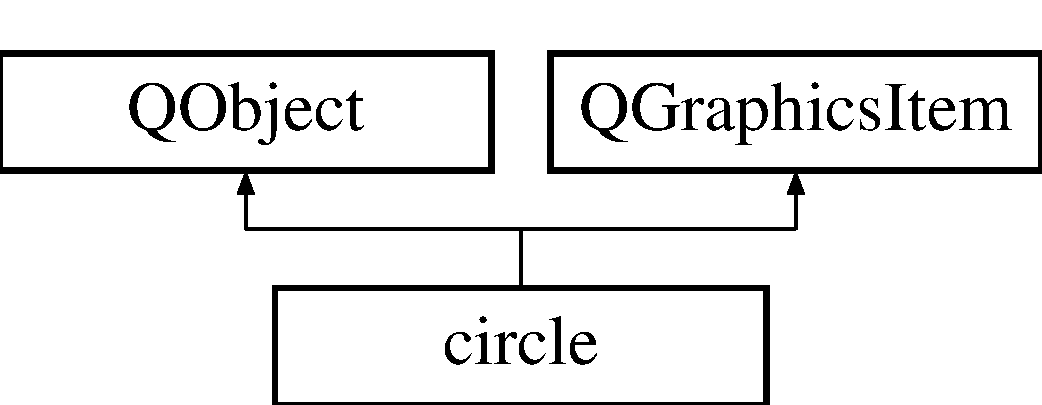
\includegraphics[height=2.000000cm]{classcircle}
\end{center}
\end{figure}
\subsection*{Public Member Functions}
\begin{DoxyCompactItemize}
\item 
\mbox{\hyperlink{classcircle_abfd721dc65145023cf14739adacc81a8}{circle}} (\mbox{\hyperlink{classgraphic_cycle}{graphic\+Cycle}} $\ast$parent, struct \mbox{\hyperlink{structcycle_data}{cycle\+Data}} data)
\begin{DoxyCompactList}\small\item\em circle\+::line Create a new circle. \end{DoxyCompactList}\item 
void \mbox{\hyperlink{classcircle_a2d9af8e86fb3605c736689a2e2566d26}{paint}} (Q\+Painter $\ast$painter, const Q\+Style\+Option\+Graphics\+Item $\ast$option, Q\+Widget $\ast$widget)
\begin{DoxyCompactList}\small\item\em \mbox{\hyperlink{classcircle_a2d9af8e86fb3605c736689a2e2566d26}{circle\+::paint}} Paint the circle on the scene. \end{DoxyCompactList}\item 
Q\+RectF \mbox{\hyperlink{classcircle_ab9d2059829ac8f0420c7e711caeb61c7}{bounding\+Rect}} () const
\begin{DoxyCompactList}\small\item\em \mbox{\hyperlink{classcircle_ab9d2059829ac8f0420c7e711caeb61c7}{circle\+::bounding\+Rect}} Define the bounding rect. \end{DoxyCompactList}\item 
Q\+Painter\+Path \mbox{\hyperlink{classcircle_a198cbcea745bd311fe91c2a23def746c}{shape}} () const
\begin{DoxyCompactList}\small\item\em \mbox{\hyperlink{classcircle_a198cbcea745bd311fe91c2a23def746c}{circle\+::shape}} Define the clipping mask of the object \end{DoxyCompactList}\end{DoxyCompactItemize}


\subsection{Constructor \& Destructor Documentation}
\mbox{\Hypertarget{classcircle_abfd721dc65145023cf14739adacc81a8}\label{classcircle_abfd721dc65145023cf14739adacc81a8}} 
\index{circle@{circle}!circle@{circle}}
\index{circle@{circle}!circle@{circle}}
\subsubsection{\texorpdfstring{circle()}{circle()}}
{\footnotesize\ttfamily circle\+::circle (\begin{DoxyParamCaption}\item[{\mbox{\hyperlink{classgraphic_cycle}{graphic\+Cycle}} $\ast$}]{parent,  }\item[{struct \mbox{\hyperlink{structcycle_data}{cycle\+Data}}}]{data }\end{DoxyParamCaption})}



circle\+::line Create a new circle. 


\begin{DoxyParams}{Parameters}
{\em struct} & \mbox{\hyperlink{structcycle_data}{cycle\+Data}} data Contains the data needed to draw the circle.\\
\hline
\end{DoxyParams}
Construct a new line on the scene and assign it to the parent \mbox{\hyperlink{classgraphic_cycle}{graphic\+Cycle}}. 

\subsection{Member Function Documentation}
\mbox{\Hypertarget{classcircle_ab9d2059829ac8f0420c7e711caeb61c7}\label{classcircle_ab9d2059829ac8f0420c7e711caeb61c7}} 
\index{circle@{circle}!bounding\+Rect@{bounding\+Rect}}
\index{bounding\+Rect@{bounding\+Rect}!circle@{circle}}
\subsubsection{\texorpdfstring{bounding\+Rect()}{boundingRect()}}
{\footnotesize\ttfamily Q\+RectF circle\+::bounding\+Rect (\begin{DoxyParamCaption}{ }\end{DoxyParamCaption}) const}



\mbox{\hyperlink{classcircle_ab9d2059829ac8f0420c7e711caeb61c7}{circle\+::bounding\+Rect}} Define the bounding rect. 

\begin{DoxyReturn}{Returns}
Q\+RectF
\end{DoxyReturn}
Define the box the object is drawn within on the scene. \mbox{\Hypertarget{classcircle_a2d9af8e86fb3605c736689a2e2566d26}\label{classcircle_a2d9af8e86fb3605c736689a2e2566d26}} 
\index{circle@{circle}!paint@{paint}}
\index{paint@{paint}!circle@{circle}}
\subsubsection{\texorpdfstring{paint()}{paint()}}
{\footnotesize\ttfamily void circle\+::paint (\begin{DoxyParamCaption}\item[{Q\+Painter $\ast$}]{painter,  }\item[{const Q\+Style\+Option\+Graphics\+Item $\ast$}]{option,  }\item[{Q\+Widget $\ast$}]{widget }\end{DoxyParamCaption})}



\mbox{\hyperlink{classcircle_a2d9af8e86fb3605c736689a2e2566d26}{circle\+::paint}} Paint the circle on the scene. 


\begin{DoxyParams}{Parameters}
{\em painter} & Q\+Painter object. \\
\hline
{\em option} & \\
\hline
{\em widget} & This function paints the point on the scene given various parameters (such as x and y). The point is drawn differently dependent on the drawing metric in use. \\
\hline
\end{DoxyParams}
\mbox{\Hypertarget{classcircle_a198cbcea745bd311fe91c2a23def746c}\label{classcircle_a198cbcea745bd311fe91c2a23def746c}} 
\index{circle@{circle}!shape@{shape}}
\index{shape@{shape}!circle@{circle}}
\subsubsection{\texorpdfstring{shape()}{shape()}}
{\footnotesize\ttfamily Q\+Painter\+Path circle\+::shape (\begin{DoxyParamCaption}{ }\end{DoxyParamCaption}) const}



\mbox{\hyperlink{classcircle_a198cbcea745bd311fe91c2a23def746c}{circle\+::shape}} Define the clipping mask of the object 

\begin{DoxyReturn}{Returns}
Q\+Painter\+Path
\end{DoxyReturn}
Defines the area in which the shape actually exists. 

The documentation for this class was generated from the following files\+:\begin{DoxyCompactItemize}
\item 
/\+Users/lukehutton/\+One\+Drive -\/ University of Leeds/\+University/\+Computer Science/\+Internship/moebinv-\/gui/include/circle.\+h\item 
/\+Users/lukehutton/\+One\+Drive -\/ University of Leeds/\+University/\+Computer Science/\+Internship/moebinv-\/gui/src/circle.\+cpp\end{DoxyCompactItemize}

\hypertarget{classcycle_context_menu}{}\section{cycle\+Context\+Menu Class Reference}
\label{classcycle_context_menu}\index{cycle\+Context\+Menu@{cycle\+Context\+Menu}}


The \mbox{\hyperlink{classcycle_context_menu}{cycle\+Context\+Menu}} class.  




{\ttfamily \#include $<$cyclecontextmenu.\+h$>$}

Inheritance diagram for cycle\+Context\+Menu\+:\begin{figure}[H]
\begin{center}
\leavevmode
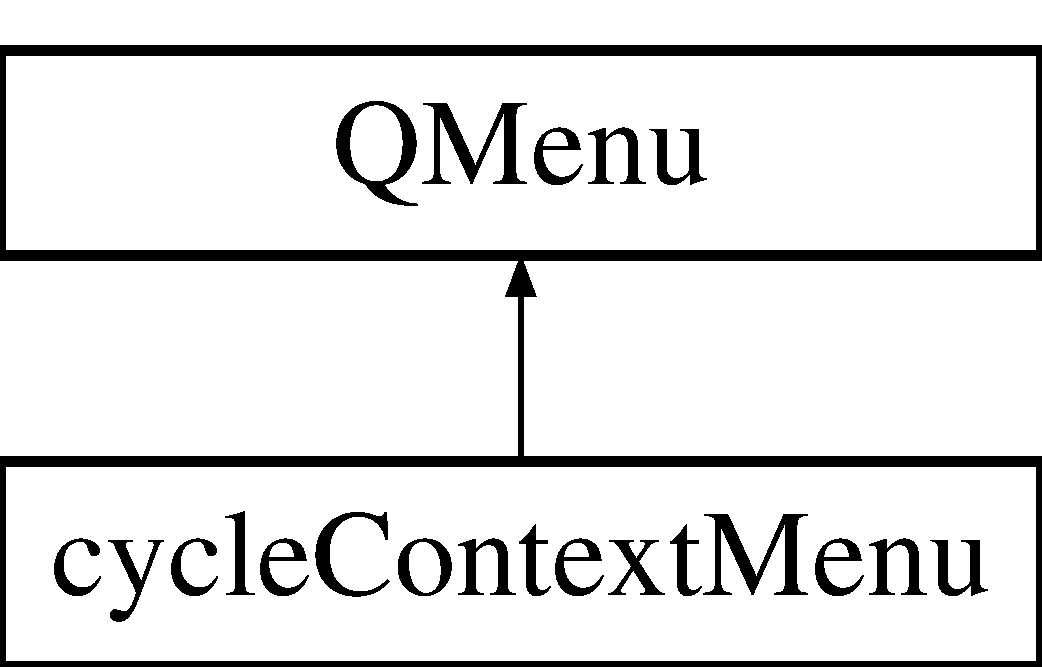
\includegraphics[height=2.000000cm]{classcycle_context_menu}
\end{center}
\end{figure}
\subsection*{Public Slots}
\begin{DoxyCompactItemize}
\item 
\mbox{\Hypertarget{classcycle_context_menu_a844d59a74d643b19fd19eb1de11ea4e9}\label{classcycle_context_menu_a844d59a74d643b19fd19eb1de11ea4e9}} 
void \mbox{\hyperlink{classcycle_context_menu_a844d59a74d643b19fd19eb1de11ea4e9}{confirm\+Delete\+Cycle}} ()
\begin{DoxyCompactList}\small\item\em \mbox{\hyperlink{classcycle_context_menu_a844d59a74d643b19fd19eb1de11ea4e9}{cycle\+Context\+Menu\+::confirm\+Delete\+Cycle}} slot that asks the user whether they would like to delete the cycle. If they select yes the cycle is deleted from the figure and the scene is updated. \end{DoxyCompactList}\item 
\mbox{\Hypertarget{classcycle_context_menu_a6a75f4ba6b3db319468db92fd0948a65}\label{classcycle_context_menu_a6a75f4ba6b3db319468db92fd0948a65}} 
void \mbox{\hyperlink{classcycle_context_menu_a6a75f4ba6b3db319468db92fd0948a65}{amend\+Relation\+List}} ()
\begin{DoxyCompactList}\small\item\em \mbox{\hyperlink{classcycle_context_menu_a6a75f4ba6b3db319468db92fd0948a65}{cycle\+Context\+Menu\+::amend\+Relation\+List}} This slot corrects the relation list after a new relation has been selected. First the sender object is identified. If the sender action is in a group then the whole of the group is searched removing any relations that are not checked (since anyone of them could have been checked before). Then the relation is added to the relation list if it has been checked and removed if it hasn\textquotesingle{}t. The relations\+Have\+Changed signal is emmitted to update the status bar text at the bottom of the application. \end{DoxyCompactList}\item 
\mbox{\Hypertarget{classcycle_context_menu_abf4f98f97561d5acd104a6c0b2038e15}\label{classcycle_context_menu_abf4f98f97561d5acd104a6c0b2038e15}} 
void \mbox{\hyperlink{classcycle_context_menu_abf4f98f97561d5acd104a6c0b2038e15}{display\+Colour\+Dialog}} ()
\begin{DoxyCompactList}\small\item\em \mbox{\hyperlink{classcycle_context_menu_abf4f98f97561d5acd104a6c0b2038e15}{cycle\+Context\+Menu\+::display\+Colour\+Dialog}} Displays the colour dialog so the user can select a colour for the cycle. \end{DoxyCompactList}\item 
\mbox{\Hypertarget{classcycle_context_menu_a094bbed14bab12e3b9ac3ae07140bdcb}\label{classcycle_context_menu_a094bbed14bab12e3b9ac3ae07140bdcb}} 
void \mbox{\hyperlink{classcycle_context_menu_a094bbed14bab12e3b9ac3ae07140bdcb}{display\+Style\+Dialog}} ()
\begin{DoxyCompactList}\small\item\em \mbox{\hyperlink{classcycle_context_menu_a094bbed14bab12e3b9ac3ae07140bdcb}{cycle\+Context\+Menu\+::display\+Style\+Dialog}} Display the style dialog so the user can select a style for the cycle. \end{DoxyCompactList}\item 
\mbox{\Hypertarget{classcycle_context_menu_ac720f89ffd13952e79dd77c1bb15c2aa}\label{classcycle_context_menu_ac720f89ffd13952e79dd77c1bb15c2aa}} 
void \mbox{\hyperlink{classcycle_context_menu_ac720f89ffd13952e79dd77c1bb15c2aa}{display\+Weight\+Dialog}} ()
\begin{DoxyCompactList}\small\item\em \mbox{\hyperlink{classcycle_context_menu_ac720f89ffd13952e79dd77c1bb15c2aa}{cycle\+Context\+Menu\+::display\+Weight\+Dialog}} Display the weight dialog so the user can select a weight for the cycle. \end{DoxyCompactList}\item 
void \mbox{\hyperlink{classcycle_context_menu_ae807f1cddefcdedf9f8c60473bd287df}{edit\+Point}} ()
\begin{DoxyCompactList}\small\item\em \mbox{\hyperlink{classcycle_context_menu_ae807f1cddefcdedf9f8c60473bd287df}{cycle\+Context\+Menu\+::edit\+Point}} \end{DoxyCompactList}\end{DoxyCompactItemize}
\subsection*{Signals}
\begin{DoxyCompactItemize}
\item 
\mbox{\Hypertarget{classcycle_context_menu_a42d360ffa2a047c3f43ded9fcec5982b}\label{classcycle_context_menu_a42d360ffa2a047c3f43ded9fcec5982b}} 
void {\bfseries relations\+Have\+Changed} ()
\item 
\mbox{\Hypertarget{classcycle_context_menu_acd8ba953b7b1edfac94b5ba4158217af}\label{classcycle_context_menu_acd8ba953b7b1edfac94b5ba4158217af}} 
void {\bfseries colour\+Selected} (Q\+Color colour)
\item 
\mbox{\Hypertarget{classcycle_context_menu_ac91d09b750dfeace9334b67649fbbda0}\label{classcycle_context_menu_ac91d09b750dfeace9334b67649fbbda0}} 
void {\bfseries weight\+Selected} (double weight)
\item 
\mbox{\Hypertarget{classcycle_context_menu_a31b1b2e1f6596697cdac2cf0cb66359e}\label{classcycle_context_menu_a31b1b2e1f6596697cdac2cf0cb66359e}} 
void {\bfseries style\+Selected} (int style)
\item 
\mbox{\Hypertarget{classcycle_context_menu_a0e28f14e9918aef074523854b5364c3e}\label{classcycle_context_menu_a0e28f14e9918aef074523854b5364c3e}} 
void {\bfseries scene\+Invalid} ()
\item 
\mbox{\Hypertarget{classcycle_context_menu_a6b92c1d84f101c8386d1152b680247ff}\label{classcycle_context_menu_a6b92c1d84f101c8386d1152b680247ff}} 
void {\bfseries changes\+Made\+To\+Figure} (const Moeb\+Inv\+::figure \&original\+Figure, const Moeb\+Inv\+::figure \&changed\+Figure)
\end{DoxyCompactItemize}
\subsection*{Public Member Functions}
\begin{DoxyCompactItemize}
\item 
\mbox{\hyperlink{classcycle_context_menu_a0a948765494ab4b2ecf73c89123f7f14}{cycle\+Context\+Menu}} (Moeb\+Inv\+::figure $\ast$f, Gi\+Na\+C\+::ex cycle, Gi\+Na\+C\+::lst $\ast$relation\+List, bool is\+Delete=true, bool is\+This=false, bool show\+Edit\+Menu=false)
\begin{DoxyCompactList}\small\item\em \mbox{\hyperlink{classcycle_context_menu_a0a948765494ab4b2ecf73c89123f7f14}{cycle\+Context\+Menu\+::cycle\+Context\+Menu}} Context menu constructor \end{DoxyCompactList}\item 
Gi\+Na\+C\+::ex \mbox{\hyperlink{classcycle_context_menu_a35b3868cdc32b97e7c4abc109ee13460}{get\+Cycle}} ()
\begin{DoxyCompactList}\small\item\em \mbox{\hyperlink{classcycle_context_menu_a35b3868cdc32b97e7c4abc109ee13460}{cycle\+Context\+Menu\+::get\+Cycle}} get cycle related to the context menu. \end{DoxyCompactList}\item 
Q\+List$<$ \mbox{\hyperlink{classmenu_rel_action}{menu\+Rel\+Action}} $\ast$ $>$ \mbox{\hyperlink{classcycle_context_menu_a4dd57e4522c46a70367b6b721f23bcc9}{get\+Actions}} ()
\begin{DoxyCompactList}\small\item\em \mbox{\hyperlink{classcycle_context_menu_a4dd57e4522c46a70367b6b721f23bcc9}{cycle\+Context\+Menu\+::get\+Actions}} get actions in the context menu. \end{DoxyCompactList}\item 
Q\+Action $\ast$ \mbox{\hyperlink{classcycle_context_menu_a0e955d1a633d3585d11b7c193341a568}{get\+Title\+Action}} ()
\begin{DoxyCompactList}\small\item\em \mbox{\hyperlink{classcycle_context_menu_a0e955d1a633d3585d11b7c193341a568}{cycle\+Context\+Menu\+::get\+Title\+Action}} get the action that will be used as the title of the context menu. This has been created due to the fact that cross compatability for \textquotesingle{}add\+Section()\textquotesingle{} isn\textquotesingle{}t well established. \end{DoxyCompactList}\item 
void \mbox{\hyperlink{classcycle_context_menu_adf29caf51604118b6ced6a02c5172252}{set\+Cycle}} (Gi\+Na\+C\+::ex cycle)
\begin{DoxyCompactList}\small\item\em \mbox{\hyperlink{classcycle_context_menu_adf29caf51604118b6ced6a02c5172252}{cycle\+Context\+Menu\+::set\+Cycle}} set the cycle that the context menu represents. \end{DoxyCompactList}\item 
void \mbox{\hyperlink{classcycle_context_menu_a83f3eb1ea5338154095a7bf1e2c77b01}{remove\+Relation\+From\+List}} (\mbox{\hyperlink{classmenu_rel_action}{menu\+Rel\+Action}} $\ast$action\+Triggered)
\begin{DoxyCompactList}\small\item\em \mbox{\hyperlink{classcycle_context_menu_a83f3eb1ea5338154095a7bf1e2c77b01}{cycle\+Context\+Menu\+::remove\+Relation\+From\+List}} This function removes a relation from the list by creating a new list and adding every item except the item that needs to be removed. The \textquotesingle{}relation\+List\textquotesingle{} from \mbox{\hyperlink{class_main_window}{Main\+Window}} is then updated so that \textquotesingle{}relation\textquotesingle{} is no longer in the list. \end{DoxyCompactList}\item 
void \mbox{\hyperlink{classcycle_context_menu_a155448ae220555423d26b055f50b6e49}{build\+Context\+Menu}} ()
\begin{DoxyCompactList}\small\item\em \mbox{\hyperlink{classcycle_context_menu_a155448ae220555423d26b055f50b6e49}{cycle\+Context\+Menu\+::build\+Context\+Menu}} Build the layout of the contextmenu. \end{DoxyCompactList}\item 
\mbox{\Hypertarget{classcycle_context_menu_a2ada1b40956db90398503d184afdd5ee}\label{classcycle_context_menu_a2ada1b40956db90398503d184afdd5ee}} 
void \mbox{\hyperlink{classcycle_context_menu_a2ada1b40956db90398503d184afdd5ee}{build\+Actions}} ()
\begin{DoxyCompactList}\small\item\em \mbox{\hyperlink{classcycle_context_menu_a2ada1b40956db90398503d184afdd5ee}{cycle\+Context\+Menu\+::build\+Actions}} initialize all the actions that will be displayed in the context menu and connect their trigger signals to slots. \end{DoxyCompactList}\item 
\mbox{\Hypertarget{classcycle_context_menu_a17d519c784fac28e39da31478b810ae9}\label{classcycle_context_menu_a17d519c784fac28e39da31478b810ae9}} 
Q\+String {\bfseries node\+\_\+label} (Gi\+Na\+C\+::ex name)
\end{DoxyCompactItemize}
\subsection*{Public Attributes}
\begin{DoxyCompactItemize}
\item 
\mbox{\Hypertarget{classcycle_context_menu_a1e2215915914b4c36463cbe5e667722d}\label{classcycle_context_menu_a1e2215915914b4c36463cbe5e667722d}} 
Q\+Pointer$<$ Q\+Action $>$ {\bfseries change\+Colour} = nullptr
\item 
\mbox{\Hypertarget{classcycle_context_menu_a61f2889cd624664ec0b4933def974a04}\label{classcycle_context_menu_a61f2889cd624664ec0b4933def974a04}} 
Q\+Pointer$<$ Q\+Action $>$ {\bfseries change\+Style} = nullptr
\item 
\mbox{\Hypertarget{classcycle_context_menu_a9798e2ec98b4e15af313112411cd8a24}\label{classcycle_context_menu_a9798e2ec98b4e15af313112411cd8a24}} 
Q\+Pointer$<$ Q\+Action $>$ {\bfseries change\+Weight} = nullptr
\item 
\mbox{\Hypertarget{classcycle_context_menu_aa58c68008bb6ab0d70af517821b8a48f}\label{classcycle_context_menu_aa58c68008bb6ab0d70af517821b8a48f}} 
Q\+Pointer$<$ Q\+Action $>$ {\bfseries delete\+Point} = nullptr
\item 
\mbox{\Hypertarget{classcycle_context_menu_a7c9b8d13930dc91c050e5b870f7dbfb8}\label{classcycle_context_menu_a7c9b8d13930dc91c050e5b870f7dbfb8}} 
Q\+Pointer$<$ Q\+Action $>$ {\bfseries edit} = nullptr
\end{DoxyCompactItemize}


\subsection{Detailed Description}
The \mbox{\hyperlink{classcycle_context_menu}{cycle\+Context\+Menu}} class. 

This class creates a context menu which is then used by each of the cycles created on the scene. It then connects each of the menu items so they function as intended. 

\subsection{Constructor \& Destructor Documentation}
\mbox{\Hypertarget{classcycle_context_menu_a0a948765494ab4b2ecf73c89123f7f14}\label{classcycle_context_menu_a0a948765494ab4b2ecf73c89123f7f14}} 
\index{cycle\+Context\+Menu@{cycle\+Context\+Menu}!cycle\+Context\+Menu@{cycle\+Context\+Menu}}
\index{cycle\+Context\+Menu@{cycle\+Context\+Menu}!cycle\+Context\+Menu@{cycle\+Context\+Menu}}
\subsubsection{\texorpdfstring{cycle\+Context\+Menu()}{cycleContextMenu()}}
{\footnotesize\ttfamily cycle\+Context\+Menu\+::cycle\+Context\+Menu (\begin{DoxyParamCaption}\item[{Moeb\+Inv\+::figure $\ast$}]{f,  }\item[{Gi\+Na\+C\+::ex}]{cycle,  }\item[{Gi\+Na\+C\+::lst $\ast$}]{relation\+List,  }\item[{bool}]{is\+Delete = {\ttfamily true},  }\item[{bool}]{is\+This = {\ttfamily false},  }\item[{bool}]{show\+Edit\+Menu = {\ttfamily false} }\end{DoxyParamCaption})}



\mbox{\hyperlink{classcycle_context_menu_a0a948765494ab4b2ecf73c89123f7f14}{cycle\+Context\+Menu\+::cycle\+Context\+Menu}} Context menu constructor 


\begin{DoxyParams}{Parameters}
{\em f} & -\/ pointer to the figure. \\
\hline
{\em cycle} & -\/ cycle the context menu is related to. \\
\hline
{\em relation\+List} & -\/ pointer to the list that stores the current selected relations from every cycle in the figure. \\
\hline
{\em is\+Delete} & -\/ does the cycle have the delete option or not? (some cycles cannot be deleted e.\+g. infy)\\
\hline
\end{DoxyParams}
Creates a cycle context menu. This allows for the selection and input of relations and allows the properties of a relation to be changed.

\subsubsection*{Current context menu\+: }

\subsubsection*{title }

standard \subsubsection*{relations }

exclusive \subsubsection*{tangent }

relations \subsubsection*{with inputs }

\subsubsection*{style }

\subsubsection*{edit }

\subsubsection*{delete }

\subsection{Member Function Documentation}
\mbox{\Hypertarget{classcycle_context_menu_a155448ae220555423d26b055f50b6e49}\label{classcycle_context_menu_a155448ae220555423d26b055f50b6e49}} 
\index{cycle\+Context\+Menu@{cycle\+Context\+Menu}!build\+Context\+Menu@{build\+Context\+Menu}}
\index{build\+Context\+Menu@{build\+Context\+Menu}!cycle\+Context\+Menu@{cycle\+Context\+Menu}}
\subsubsection{\texorpdfstring{build\+Context\+Menu()}{buildContextMenu()}}
{\footnotesize\ttfamily void cycle\+Context\+Menu\+::build\+Context\+Menu (\begin{DoxyParamCaption}{ }\end{DoxyParamCaption})}



\mbox{\hyperlink{classcycle_context_menu_a155448ae220555423d26b055f50b6e49}{cycle\+Context\+Menu\+::build\+Context\+Menu}} Build the layout of the contextmenu. 

Note\+: If a new relation or action is added this layout function will need to be adapted to suit the new layout. \mbox{\Hypertarget{classcycle_context_menu_ae807f1cddefcdedf9f8c60473bd287df}\label{classcycle_context_menu_ae807f1cddefcdedf9f8c60473bd287df}} 
\index{cycle\+Context\+Menu@{cycle\+Context\+Menu}!edit\+Point@{edit\+Point}}
\index{edit\+Point@{edit\+Point}!cycle\+Context\+Menu@{cycle\+Context\+Menu}}
\subsubsection{\texorpdfstring{edit\+Point}{editPoint}}
{\footnotesize\ttfamily void cycle\+Context\+Menu\+::edit\+Point (\begin{DoxyParamCaption}{ }\end{DoxyParamCaption})\hspace{0.3cm}{\ttfamily [slot]}}



\mbox{\hyperlink{classcycle_context_menu_ae807f1cddefcdedf9f8c60473bd287df}{cycle\+Context\+Menu\+::edit\+Point}} 

Displays a dialog that allows you to edit a point of generation 0. This dialog lets you enter the values k, l, n, m or (x, y) and radius squared to edit a point. \mbox{\Hypertarget{classcycle_context_menu_a4dd57e4522c46a70367b6b721f23bcc9}\label{classcycle_context_menu_a4dd57e4522c46a70367b6b721f23bcc9}} 
\index{cycle\+Context\+Menu@{cycle\+Context\+Menu}!get\+Actions@{get\+Actions}}
\index{get\+Actions@{get\+Actions}!cycle\+Context\+Menu@{cycle\+Context\+Menu}}
\subsubsection{\texorpdfstring{get\+Actions()}{getActions()}}
{\footnotesize\ttfamily Q\+List$<$ \mbox{\hyperlink{classmenu_rel_action}{menu\+Rel\+Action}} $\ast$ $>$ cycle\+Context\+Menu\+::get\+Actions (\begin{DoxyParamCaption}{ }\end{DoxyParamCaption})}



\mbox{\hyperlink{classcycle_context_menu_a4dd57e4522c46a70367b6b721f23bcc9}{cycle\+Context\+Menu\+::get\+Actions}} get actions in the context menu. 

\begin{DoxyReturn}{Returns}
Q\+List$<$menu\+Rel\+Action $\ast$$>$ list of \mbox{\hyperlink{classmenu_rel_action}{menu\+Rel\+Action}} pointers. 
\end{DoxyReturn}
\mbox{\Hypertarget{classcycle_context_menu_a35b3868cdc32b97e7c4abc109ee13460}\label{classcycle_context_menu_a35b3868cdc32b97e7c4abc109ee13460}} 
\index{cycle\+Context\+Menu@{cycle\+Context\+Menu}!get\+Cycle@{get\+Cycle}}
\index{get\+Cycle@{get\+Cycle}!cycle\+Context\+Menu@{cycle\+Context\+Menu}}
\subsubsection{\texorpdfstring{get\+Cycle()}{getCycle()}}
{\footnotesize\ttfamily ex cycle\+Context\+Menu\+::get\+Cycle (\begin{DoxyParamCaption}{ }\end{DoxyParamCaption})}



\mbox{\hyperlink{classcycle_context_menu_a35b3868cdc32b97e7c4abc109ee13460}{cycle\+Context\+Menu\+::get\+Cycle}} get cycle related to the context menu. 

\begin{DoxyReturn}{Returns}
Gi\+Na\+C\+::ex. 
\end{DoxyReturn}
\mbox{\Hypertarget{classcycle_context_menu_a0e955d1a633d3585d11b7c193341a568}\label{classcycle_context_menu_a0e955d1a633d3585d11b7c193341a568}} 
\index{cycle\+Context\+Menu@{cycle\+Context\+Menu}!get\+Title\+Action@{get\+Title\+Action}}
\index{get\+Title\+Action@{get\+Title\+Action}!cycle\+Context\+Menu@{cycle\+Context\+Menu}}
\subsubsection{\texorpdfstring{get\+Title\+Action()}{getTitleAction()}}
{\footnotesize\ttfamily Q\+Action $\ast$ cycle\+Context\+Menu\+::get\+Title\+Action (\begin{DoxyParamCaption}{ }\end{DoxyParamCaption})}



\mbox{\hyperlink{classcycle_context_menu_a0e955d1a633d3585d11b7c193341a568}{cycle\+Context\+Menu\+::get\+Title\+Action}} get the action that will be used as the title of the context menu. This has been created due to the fact that cross compatability for \textquotesingle{}add\+Section()\textquotesingle{} isn\textquotesingle{}t well established. 

\begin{DoxyReturn}{Returns}
Q\+Action$\ast$ -\/ A pointer to the Q\+Action. 
\end{DoxyReturn}
\mbox{\Hypertarget{classcycle_context_menu_a83f3eb1ea5338154095a7bf1e2c77b01}\label{classcycle_context_menu_a83f3eb1ea5338154095a7bf1e2c77b01}} 
\index{cycle\+Context\+Menu@{cycle\+Context\+Menu}!remove\+Relation\+From\+List@{remove\+Relation\+From\+List}}
\index{remove\+Relation\+From\+List@{remove\+Relation\+From\+List}!cycle\+Context\+Menu@{cycle\+Context\+Menu}}
\subsubsection{\texorpdfstring{remove\+Relation\+From\+List()}{removeRelationFromList()}}
{\footnotesize\ttfamily void cycle\+Context\+Menu\+::remove\+Relation\+From\+List (\begin{DoxyParamCaption}\item[{\mbox{\hyperlink{classmenu_rel_action}{menu\+Rel\+Action}} $\ast$}]{action\+Triggered }\end{DoxyParamCaption})}



\mbox{\hyperlink{classcycle_context_menu_a83f3eb1ea5338154095a7bf1e2c77b01}{cycle\+Context\+Menu\+::remove\+Relation\+From\+List}} This function removes a relation from the list by creating a new list and adding every item except the item that needs to be removed. The \textquotesingle{}relation\+List\textquotesingle{} from \mbox{\hyperlink{class_main_window}{Main\+Window}} is then updated so that \textquotesingle{}relation\textquotesingle{} is no longer in the list. 


\begin{DoxyParams}{Parameters}
{\em relation} & -\/ the cycle\+\_\+relation that is to be removed. \\
\hline
\end{DoxyParams}
\mbox{\Hypertarget{classcycle_context_menu_adf29caf51604118b6ced6a02c5172252}\label{classcycle_context_menu_adf29caf51604118b6ced6a02c5172252}} 
\index{cycle\+Context\+Menu@{cycle\+Context\+Menu}!set\+Cycle@{set\+Cycle}}
\index{set\+Cycle@{set\+Cycle}!cycle\+Context\+Menu@{cycle\+Context\+Menu}}
\subsubsection{\texorpdfstring{set\+Cycle()}{setCycle()}}
{\footnotesize\ttfamily void cycle\+Context\+Menu\+::set\+Cycle (\begin{DoxyParamCaption}\item[{Gi\+Na\+C\+::ex}]{cycle }\end{DoxyParamCaption})}



\mbox{\hyperlink{classcycle_context_menu_adf29caf51604118b6ced6a02c5172252}{cycle\+Context\+Menu\+::set\+Cycle}} set the cycle that the context menu represents. 


\begin{DoxyParams}{Parameters}
{\em cycle} & -\/ the cycle in which the context menu will be \textquotesingle{}linked\textquotesingle{} to. \\
\hline
\end{DoxyParams}


The documentation for this class was generated from the following files\+:\begin{DoxyCompactItemize}
\item 
/\+Users/lukehutton/\+One\+Drive -\/ University of Leeds/\+University/\+Computer Science/\+Internship/moebinv-\/gui/include/cyclecontextmenu.\+h\item 
/\+Users/lukehutton/\+One\+Drive -\/ University of Leeds/\+University/\+Computer Science/\+Internship/moebinv-\/gui/src/cyclecontextmenu.\+cpp\end{DoxyCompactItemize}

\hypertarget{classgraphic_cycle}{}\section{graphic\+Cycle Class Reference}
\label{classgraphic_cycle}\index{graphic\+Cycle@{graphic\+Cycle}}


The \mbox{\hyperlink{classgraphic_cycle}{graphic\+Cycle}} class.  




{\ttfamily \#include $<$graphiccycle.\+h$>$}

Inheritance diagram for graphic\+Cycle\+:\begin{figure}[H]
\begin{center}
\leavevmode
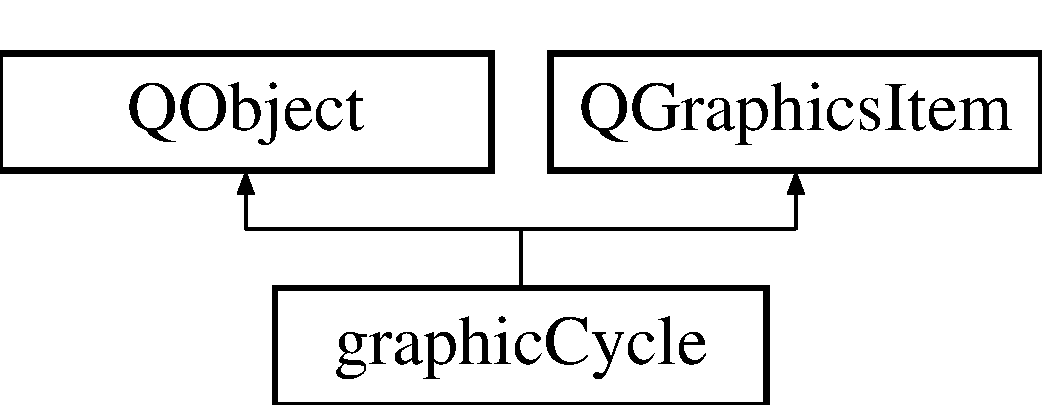
\includegraphics[height=2.000000cm]{classgraphic_cycle}
\end{center}
\end{figure}
\subsection*{Public Slots}
\begin{DoxyCompactItemize}
\item 
void \mbox{\hyperlink{classgraphic_cycle_a54708026fc7ea647f431263990872cdf}{set\+Hover}} ()
\begin{DoxyCompactList}\small\item\em \mbox{\hyperlink{classgraphic_cycle_a54708026fc7ea647f431263990872cdf}{graphic\+Cycle\+::set\+Hover}} set the hover style of the object. \end{DoxyCompactList}\item 
void \mbox{\hyperlink{classgraphic_cycle_a7d9d805ccc83dcf16623c969ad48b6a5}{unset\+Hover}} ()
\begin{DoxyCompactList}\small\item\em \mbox{\hyperlink{classgraphic_cycle_a7d9d805ccc83dcf16623c969ad48b6a5}{graphic\+Cycle\+::unset\+Hover}} unset the object hover \end{DoxyCompactList}\item 
void \mbox{\hyperlink{classgraphic_cycle_a48965c220e8fad0181f1f793c17fb73c}{set\+Colour}} (Q\+Color colour)
\begin{DoxyCompactList}\small\item\em \mbox{\hyperlink{classgraphic_cycle_a48965c220e8fad0181f1f793c17fb73c}{graphic\+Cycle\+::set\+Colour}} set the colour of the graphic cycle. \end{DoxyCompactList}\item 
void \mbox{\hyperlink{classgraphic_cycle_aa02ce6a22ddb0ae859ab6dac49a0570a}{set\+Line\+Width}} (double weight)
\begin{DoxyCompactList}\small\item\em \mbox{\hyperlink{classgraphic_cycle_aa02ce6a22ddb0ae859ab6dac49a0570a}{graphic\+Cycle\+::set\+Line\+Width}} set the weight of the graphic cycle. \end{DoxyCompactList}\item 
void \mbox{\hyperlink{classgraphic_cycle_a96f1a1d6c958bfba3789a13c156f9795}{set\+Line\+Style}} (int style)
\begin{DoxyCompactList}\small\item\em \mbox{\hyperlink{classgraphic_cycle_a96f1a1d6c958bfba3789a13c156f9795}{graphic\+Cycle\+::set\+Line\+Style}} set the style of the graphic cycle. \end{DoxyCompactList}\item 
void \mbox{\hyperlink{classgraphic_cycle_a173e5e3dfb0dde41c8046a53086e02ab}{mouse\+Stopped}} ()
\begin{DoxyCompactList}\small\item\em \mbox{\hyperlink{classgraphic_cycle_a173e5e3dfb0dde41c8046a53086e02ab}{graphic\+Cycle\+::mouse\+Stopped}} \end{DoxyCompactList}\item 
void \mbox{\hyperlink{classgraphic_cycle_af79bfc4ed813bab595a2a721475a7199}{cancel\+Movement}} ()
\begin{DoxyCompactList}\small\item\em \mbox{\hyperlink{classgraphic_cycle_af79bfc4ed813bab595a2a721475a7199}{graphic\+Cycle\+::cancel\+Movement}} \end{DoxyCompactList}\end{DoxyCompactItemize}
\subsection*{Signals}
\begin{DoxyCompactItemize}
\item 
\mbox{\Hypertarget{classgraphic_cycle_ae60f6c55734308b7811d0f5ff9116227}\label{classgraphic_cycle_ae60f6c55734308b7811d0f5ff9116227}} 
void {\bfseries find\+Cycle\+In\+Tree} (Gi\+Na\+C\+::ex cycle)
\item 
\mbox{\Hypertarget{classgraphic_cycle_aa36164d21bdd1b7cde5b26407f330d49}\label{classgraphic_cycle_aa36164d21bdd1b7cde5b26407f330d49}} 
void {\bfseries scene\+Invalid} ()
\item 
\mbox{\Hypertarget{classgraphic_cycle_a04f2deb84f4a748e8bb9dba7a43eb653}\label{classgraphic_cycle_a04f2deb84f4a748e8bb9dba7a43eb653}} 
void {\bfseries changes\+Made\+To\+Figure} (const Moeb\+Inv\+::figure \&original\+Figure, const Moeb\+Inv\+::figure \&changed\+Figure)
\end{DoxyCompactItemize}
\subsection*{Public Member Functions}
\begin{DoxyCompactItemize}
\item 
\mbox{\hyperlink{classgraphic_cycle_a89c2914fab32a0e10b2d53491535c173}{graphic\+Cycle}} (Moeb\+Inv\+::figure $\ast$f, Gi\+Na\+C\+::ex c, double $\ast$relative\+Scale\+Factor, \mbox{\hyperlink{classcycle_context_menu}{cycle\+Context\+Menu}} $\ast$menu, struct \mbox{\hyperlink{structcycle_style_data}{cycle\+Style\+Data}} style\+Data)
\begin{DoxyCompactList}\small\item\em \mbox{\hyperlink{classgraphic_cycle_a89c2914fab32a0e10b2d53491535c173}{graphic\+Cycle\+::graphic\+Cycle}} graphicd cycle constructor. \end{DoxyCompactList}\item 
Q\+String \mbox{\hyperlink{classgraphic_cycle_ae55bb7487a8baac738b88e8c1bd0515e}{get\+Cycle\+Label}} ()
\begin{DoxyCompactList}\small\item\em \mbox{\hyperlink{classgraphic_cycle_ae55bb7487a8baac738b88e8c1bd0515e}{graphic\+Cycle\+::get\+Cycle\+Label}} get the cycle label. \end{DoxyCompactList}\item 
double $\ast$ \mbox{\hyperlink{classgraphic_cycle_a80b533c2477a08f98506202d94bad7bc}{get\+Relative\+Scale\+Factor}} ()
\begin{DoxyCompactList}\small\item\em \mbox{\hyperlink{classgraphic_cycle_a80b533c2477a08f98506202d94bad7bc}{graphic\+Cycle\+::get\+Relative\+Scale\+Factor}} get the scale factor of the scene. \end{DoxyCompactList}\item 
\mbox{\hyperlink{classcycle_context_menu}{cycle\+Context\+Menu}} $\ast$ \mbox{\hyperlink{classgraphic_cycle_a4e090d82ba2e37bee415c95630abe061}{get\+Context\+Menu}} ()
\begin{DoxyCompactList}\small\item\em \mbox{\hyperlink{classgraphic_cycle_a4e090d82ba2e37bee415c95630abe061}{graphic\+Cycle\+::get\+Context\+Menu}} get the context menu linked to the scene. \end{DoxyCompactList}\item 
\mbox{\Hypertarget{classgraphic_cycle_a10e61352945ca9b32b83e528e2fc6853}\label{classgraphic_cycle_a10e61352945ca9b32b83e528e2fc6853}} 
bool \mbox{\hyperlink{classgraphic_cycle_a10e61352945ca9b32b83e528e2fc6853}{get\+Item\+Is\+Grabbed}} ()
\begin{DoxyCompactList}\small\item\em \mbox{\hyperlink{classgraphic_cycle_a10e61352945ca9b32b83e528e2fc6853}{graphic\+Cycle\+::get\+Item\+Is\+Grabbed}} get whether the item is being moved. \end{DoxyCompactList}\item 
void \mbox{\hyperlink{classgraphic_cycle_a44dc93e5f66707fd102c2acccbef076c}{add\+Child}} (int child\+Type, const double \&x, const double \&y, const double \&c=0, const double \&radius=0)
\begin{DoxyCompactList}\small\item\em \mbox{\hyperlink{classgraphic_cycle_a44dc93e5f66707fd102c2acccbef076c}{graphic\+Cycle\+::add\+Child}} Add a new child to graphic cycle. \end{DoxyCompactList}\item 
virtual void \mbox{\hyperlink{classgraphic_cycle_a746393c5d92838147094dadee5c289f5}{paint}} (Q\+Painter $\ast$painter, const Q\+Style\+Option\+Graphics\+Item $\ast$option, Q\+Widget $\ast$widget)
\begin{DoxyCompactList}\small\item\em \mbox{\hyperlink{classgraphic_cycle_a746393c5d92838147094dadee5c289f5}{graphic\+Cycle\+::paint}} Paint the object to the scene. \end{DoxyCompactList}\item 
virtual Q\+RectF \mbox{\hyperlink{classgraphic_cycle_a4db310e0fdbccffefc7404c47eb73607}{bounding\+Rect}} () const
\begin{DoxyCompactList}\small\item\em \mbox{\hyperlink{classgraphic_cycle_a4db310e0fdbccffefc7404c47eb73607}{graphic\+Cycle\+::bounding\+Rect}} Define the bounding rect. \end{DoxyCompactList}\item 
void \mbox{\hyperlink{classgraphic_cycle_af731c349d665b784291187ad4b0a71d9}{mouse\+Press\+Event}} (Q\+Graphics\+Scene\+Mouse\+Event $\ast$event)
\begin{DoxyCompactList}\small\item\em \mbox{\hyperlink{classgraphic_cycle_af731c349d665b784291187ad4b0a71d9}{graphic\+Cycle\+::mouse\+Press\+Event}} reimplements mouse press event. \end{DoxyCompactList}\item 
void \mbox{\hyperlink{classgraphic_cycle_aec6514c9578de68150bf2eea9b4e80c4}{mouse\+Move\+Event}} (Q\+Graphics\+Scene\+Mouse\+Event $\ast$event)
\begin{DoxyCompactList}\small\item\em \mbox{\hyperlink{classgraphic_cycle_aec6514c9578de68150bf2eea9b4e80c4}{graphic\+Cycle\+::mouse\+Move\+Event}} \end{DoxyCompactList}\item 
void \mbox{\hyperlink{classgraphic_cycle_a10c7318e9cf6d79e0aad3eec5c1d697a}{mouse\+Release\+Event}} (Q\+Graphics\+Scene\+Mouse\+Event $\ast$event)
\begin{DoxyCompactList}\small\item\em \mbox{\hyperlink{classgraphic_cycle_a10c7318e9cf6d79e0aad3eec5c1d697a}{graphic\+Cycle\+::mouse\+Release\+Event}} reimplements the mouse release event. \end{DoxyCompactList}\item 
void \mbox{\hyperlink{classgraphic_cycle_ac3a007a95334380db1bcd9b8082cb36c}{build\+Shape}} ()
\begin{DoxyCompactList}\small\item\em \mbox{\hyperlink{classgraphic_cycle_ac3a007a95334380db1bcd9b8082cb36c}{graphic\+Cycle\+::build\+Shape}} build the shape. \end{DoxyCompactList}\item 
Q\+Matrix \mbox{\hyperlink{classgraphic_cycle_a1c3a094ad53a3705019c24869340ed51}{stable\+Matrix}} (const Q\+Matrix \&matrix, const Q\+PointF \&p)
\begin{DoxyCompactList}\small\item\em \mbox{\hyperlink{classgraphic_cycle_a1c3a094ad53a3705019c24869340ed51}{graphic\+Cycle\+::stable\+Matrix}} create new transformation matrix \end{DoxyCompactList}\item 
\mbox{\Hypertarget{classgraphic_cycle_a58385898752cac06fb14fc527f908b8c}\label{classgraphic_cycle_a58385898752cac06fb14fc527f908b8c}} 
bool {\bfseries set\+Cycle\+Asy} (const Gi\+Na\+C\+::ex \&new\+\_\+cycle, const struct \mbox{\hyperlink{structcycle_style_data}{cycle\+Style\+Data}} \&data)
\item 
\mbox{\Hypertarget{classgraphic_cycle_a51c0fcf1c2b413a20113c0b4e10194d9}\label{classgraphic_cycle_a51c0fcf1c2b413a20113c0b4e10194d9}} 
Q\+String {\bfseries node\+\_\+label} (Gi\+Na\+C\+::ex name)
\end{DoxyCompactItemize}


\subsection{Detailed Description}
The \mbox{\hyperlink{classgraphic_cycle}{graphic\+Cycle}} class. 

This class is the base class for all objects drawn on the scene. It contains common fucntions used by a point, circle and line drawing methods.

Inherits both Q\+Object and Q\+Graphics\+Item. 

\subsection{Constructor \& Destructor Documentation}
\mbox{\Hypertarget{classgraphic_cycle_a89c2914fab32a0e10b2d53491535c173}\label{classgraphic_cycle_a89c2914fab32a0e10b2d53491535c173}} 
\index{graphic\+Cycle@{graphic\+Cycle}!graphic\+Cycle@{graphic\+Cycle}}
\index{graphic\+Cycle@{graphic\+Cycle}!graphic\+Cycle@{graphic\+Cycle}}
\subsubsection{\texorpdfstring{graphic\+Cycle()}{graphicCycle()}}
{\footnotesize\ttfamily graphic\+Cycle\+::graphic\+Cycle (\begin{DoxyParamCaption}\item[{Moeb\+Inv\+::figure $\ast$}]{f,  }\item[{Gi\+Na\+C\+::ex}]{c,  }\item[{double $\ast$}]{relative\+Scale\+Factor,  }\item[{\mbox{\hyperlink{classcycle_context_menu}{cycle\+Context\+Menu}} $\ast$}]{menu,  }\item[{struct \mbox{\hyperlink{structcycle_style_data}{cycle\+Style\+Data}}}]{style\+Data }\end{DoxyParamCaption})}



\mbox{\hyperlink{classgraphic_cycle_a89c2914fab32a0e10b2d53491535c173}{graphic\+Cycle\+::graphic\+Cycle}} graphicd cycle constructor. 


\begin{DoxyParams}{Parameters}
{\em f} & Moeb\+Inv\+::figure \\
\hline
{\em c} & Gi\+Na\+C\+::ex the cycle that the \mbox{\hyperlink{classgraphic_cycle}{graphic\+Cycle}} represents. \\
\hline
{\em relative\+Scale\+Factor} & the scale factor of the scene. \\
\hline
{\em menu} & the menu that the graphic cycle is linked to. \\
\hline
{\em style\+Data} & the data to style the graphic cycle such as colour. \\
\hline
\end{DoxyParams}


\subsection{Member Function Documentation}
\mbox{\Hypertarget{classgraphic_cycle_a44dc93e5f66707fd102c2acccbef076c}\label{classgraphic_cycle_a44dc93e5f66707fd102c2acccbef076c}} 
\index{graphic\+Cycle@{graphic\+Cycle}!add\+Child@{add\+Child}}
\index{add\+Child@{add\+Child}!graphic\+Cycle@{graphic\+Cycle}}
\subsubsection{\texorpdfstring{add\+Child()}{addChild()}}
{\footnotesize\ttfamily void graphic\+Cycle\+::add\+Child (\begin{DoxyParamCaption}\item[{int}]{child\+Type,  }\item[{const double \&}]{x,  }\item[{const double \&}]{y,  }\item[{const double \&}]{c = {\ttfamily 0},  }\item[{const double \&}]{radius = {\ttfamily 0} }\end{DoxyParamCaption})}



\mbox{\hyperlink{classgraphic_cycle_a44dc93e5f66707fd102c2acccbef076c}{graphic\+Cycle\+::add\+Child}} Add a new child to graphic cycle. 


\begin{DoxyParams}{Parameters}
{\em child\+Type} & the type of child object to be drawn e.\+g. point, circle, line. \\
\hline
{\em x} & the x value the object will be drawn at. \\
\hline
{\em y} & the y value the object will be drawn at. \\
\hline
{\em c} & the value of c (for lines). \\
\hline
{\em radius} & the radius of the object (for circles).\\
\hline
\end{DoxyParams}
Add a new child to this graphic cycle. This could consist of any type in the enum \textquotesingle{}child\+Type\textquotesingle{}. \mbox{\Hypertarget{classgraphic_cycle_a4db310e0fdbccffefc7404c47eb73607}\label{classgraphic_cycle_a4db310e0fdbccffefc7404c47eb73607}} 
\index{graphic\+Cycle@{graphic\+Cycle}!bounding\+Rect@{bounding\+Rect}}
\index{bounding\+Rect@{bounding\+Rect}!graphic\+Cycle@{graphic\+Cycle}}
\subsubsection{\texorpdfstring{bounding\+Rect()}{boundingRect()}}
{\footnotesize\ttfamily Q\+RectF graphic\+Cycle\+::bounding\+Rect (\begin{DoxyParamCaption}{ }\end{DoxyParamCaption}) const\hspace{0.3cm}{\ttfamily [virtual]}}



\mbox{\hyperlink{classgraphic_cycle_a4db310e0fdbccffefc7404c47eb73607}{graphic\+Cycle\+::bounding\+Rect}} Define the bounding rect. 

\begin{DoxyReturn}{Returns}
Q\+RectF
\end{DoxyReturn}
Define the box the object is drawn within on the scene. This is done by getting all of the children bounding rectangles and combining them. \mbox{\Hypertarget{classgraphic_cycle_ac3a007a95334380db1bcd9b8082cb36c}\label{classgraphic_cycle_ac3a007a95334380db1bcd9b8082cb36c}} 
\index{graphic\+Cycle@{graphic\+Cycle}!build\+Shape@{build\+Shape}}
\index{build\+Shape@{build\+Shape}!graphic\+Cycle@{graphic\+Cycle}}
\subsubsection{\texorpdfstring{build\+Shape()}{buildShape()}}
{\footnotesize\ttfamily void graphic\+Cycle\+::build\+Shape (\begin{DoxyParamCaption}{ }\end{DoxyParamCaption})}



\mbox{\hyperlink{classgraphic_cycle_ac3a007a95334380db1bcd9b8082cb36c}{graphic\+Cycle\+::build\+Shape}} build the shape. 

Build the shape by adding the necessary children to the graphic cycle. If any child cannot be drawn graphically then Moeb\+Inv will thow an exception, this is caught and a message is shown in the debugger. \mbox{\Hypertarget{classgraphic_cycle_af79bfc4ed813bab595a2a721475a7199}\label{classgraphic_cycle_af79bfc4ed813bab595a2a721475a7199}} 
\index{graphic\+Cycle@{graphic\+Cycle}!cancel\+Movement@{cancel\+Movement}}
\index{cancel\+Movement@{cancel\+Movement}!graphic\+Cycle@{graphic\+Cycle}}
\subsubsection{\texorpdfstring{cancel\+Movement}{cancelMovement}}
{\footnotesize\ttfamily void graphic\+Cycle\+::cancel\+Movement (\begin{DoxyParamCaption}{ }\end{DoxyParamCaption})\hspace{0.3cm}{\ttfamily [slot]}}



\mbox{\hyperlink{classgraphic_cycle_af79bfc4ed813bab595a2a721475a7199}{graphic\+Cycle\+::cancel\+Movement}} 

Cancels a movement when a generation 0 has been grabbed and is currently being moved. \mbox{\Hypertarget{classgraphic_cycle_a4e090d82ba2e37bee415c95630abe061}\label{classgraphic_cycle_a4e090d82ba2e37bee415c95630abe061}} 
\index{graphic\+Cycle@{graphic\+Cycle}!get\+Context\+Menu@{get\+Context\+Menu}}
\index{get\+Context\+Menu@{get\+Context\+Menu}!graphic\+Cycle@{graphic\+Cycle}}
\subsubsection{\texorpdfstring{get\+Context\+Menu()}{getContextMenu()}}
{\footnotesize\ttfamily \mbox{\hyperlink{classcycle_context_menu}{cycle\+Context\+Menu}} $\ast$ graphic\+Cycle\+::get\+Context\+Menu (\begin{DoxyParamCaption}{ }\end{DoxyParamCaption})}



\mbox{\hyperlink{classgraphic_cycle_a4e090d82ba2e37bee415c95630abe061}{graphic\+Cycle\+::get\+Context\+Menu}} get the context menu linked to the scene. 

\begin{DoxyReturn}{Returns}
cycle\+Context\+Menu$\ast$ 
\end{DoxyReturn}
\mbox{\Hypertarget{classgraphic_cycle_ae55bb7487a8baac738b88e8c1bd0515e}\label{classgraphic_cycle_ae55bb7487a8baac738b88e8c1bd0515e}} 
\index{graphic\+Cycle@{graphic\+Cycle}!get\+Cycle\+Label@{get\+Cycle\+Label}}
\index{get\+Cycle\+Label@{get\+Cycle\+Label}!graphic\+Cycle@{graphic\+Cycle}}
\subsubsection{\texorpdfstring{get\+Cycle\+Label()}{getCycleLabel()}}
{\footnotesize\ttfamily Q\+String graphic\+Cycle\+::get\+Cycle\+Label (\begin{DoxyParamCaption}{ }\end{DoxyParamCaption})}



\mbox{\hyperlink{classgraphic_cycle_ae55bb7487a8baac738b88e8c1bd0515e}{graphic\+Cycle\+::get\+Cycle\+Label}} get the cycle label. 

\begin{DoxyReturn}{Returns}
Q\+String 
\end{DoxyReturn}
\mbox{\Hypertarget{classgraphic_cycle_a80b533c2477a08f98506202d94bad7bc}\label{classgraphic_cycle_a80b533c2477a08f98506202d94bad7bc}} 
\index{graphic\+Cycle@{graphic\+Cycle}!get\+Relative\+Scale\+Factor@{get\+Relative\+Scale\+Factor}}
\index{get\+Relative\+Scale\+Factor@{get\+Relative\+Scale\+Factor}!graphic\+Cycle@{graphic\+Cycle}}
\subsubsection{\texorpdfstring{get\+Relative\+Scale\+Factor()}{getRelativeScaleFactor()}}
{\footnotesize\ttfamily double $\ast$ graphic\+Cycle\+::get\+Relative\+Scale\+Factor (\begin{DoxyParamCaption}{ }\end{DoxyParamCaption})}



\mbox{\hyperlink{classgraphic_cycle_a80b533c2477a08f98506202d94bad7bc}{graphic\+Cycle\+::get\+Relative\+Scale\+Factor}} get the scale factor of the scene. 

\begin{DoxyReturn}{Returns}
double$\ast$ 
\end{DoxyReturn}
\mbox{\Hypertarget{classgraphic_cycle_aec6514c9578de68150bf2eea9b4e80c4}\label{classgraphic_cycle_aec6514c9578de68150bf2eea9b4e80c4}} 
\index{graphic\+Cycle@{graphic\+Cycle}!mouse\+Move\+Event@{mouse\+Move\+Event}}
\index{mouse\+Move\+Event@{mouse\+Move\+Event}!graphic\+Cycle@{graphic\+Cycle}}
\subsubsection{\texorpdfstring{mouse\+Move\+Event()}{mouseMoveEvent()}}
{\footnotesize\ttfamily void graphic\+Cycle\+::mouse\+Move\+Event (\begin{DoxyParamCaption}\item[{Q\+Graphics\+Scene\+Mouse\+Event $\ast$}]{event }\end{DoxyParamCaption})}



\mbox{\hyperlink{classgraphic_cycle_aec6514c9578de68150bf2eea9b4e80c4}{graphic\+Cycle\+::mouse\+Move\+Event}} 


\begin{DoxyParams}{Parameters}
{\em event} & Detect whether the mouse has been moved. \\
\hline
\end{DoxyParams}
\mbox{\Hypertarget{classgraphic_cycle_af731c349d665b784291187ad4b0a71d9}\label{classgraphic_cycle_af731c349d665b784291187ad4b0a71d9}} 
\index{graphic\+Cycle@{graphic\+Cycle}!mouse\+Press\+Event@{mouse\+Press\+Event}}
\index{mouse\+Press\+Event@{mouse\+Press\+Event}!graphic\+Cycle@{graphic\+Cycle}}
\subsubsection{\texorpdfstring{mouse\+Press\+Event()}{mousePressEvent()}}
{\footnotesize\ttfamily void graphic\+Cycle\+::mouse\+Press\+Event (\begin{DoxyParamCaption}\item[{Q\+Graphics\+Scene\+Mouse\+Event $\ast$}]{event }\end{DoxyParamCaption})}



\mbox{\hyperlink{classgraphic_cycle_af731c349d665b784291187ad4b0a71d9}{graphic\+Cycle\+::mouse\+Press\+Event}} reimplements mouse press event. 


\begin{DoxyParams}{Parameters}
{\em event} & mouse event.\\
\hline
\end{DoxyParams}
Reimplements mouse press event to allow movement of a point when it is highlighted. \mbox{\Hypertarget{classgraphic_cycle_a10c7318e9cf6d79e0aad3eec5c1d697a}\label{classgraphic_cycle_a10c7318e9cf6d79e0aad3eec5c1d697a}} 
\index{graphic\+Cycle@{graphic\+Cycle}!mouse\+Release\+Event@{mouse\+Release\+Event}}
\index{mouse\+Release\+Event@{mouse\+Release\+Event}!graphic\+Cycle@{graphic\+Cycle}}
\subsubsection{\texorpdfstring{mouse\+Release\+Event()}{mouseReleaseEvent()}}
{\footnotesize\ttfamily void graphic\+Cycle\+::mouse\+Release\+Event (\begin{DoxyParamCaption}\item[{Q\+Graphics\+Scene\+Mouse\+Event $\ast$}]{event }\end{DoxyParamCaption})}



\mbox{\hyperlink{classgraphic_cycle_a10c7318e9cf6d79e0aad3eec5c1d697a}{graphic\+Cycle\+::mouse\+Release\+Event}} reimplements the mouse release event. 


\begin{DoxyParams}{Parameters}
{\em event} & mouse event.\\
\hline
\end{DoxyParams}
Reimplements the mouse release event to allow movement of a point when it is highlighted. \mbox{\Hypertarget{classgraphic_cycle_a173e5e3dfb0dde41c8046a53086e02ab}\label{classgraphic_cycle_a173e5e3dfb0dde41c8046a53086e02ab}} 
\index{graphic\+Cycle@{graphic\+Cycle}!mouse\+Stopped@{mouse\+Stopped}}
\index{mouse\+Stopped@{mouse\+Stopped}!graphic\+Cycle@{graphic\+Cycle}}
\subsubsection{\texorpdfstring{mouse\+Stopped}{mouseStopped}}
{\footnotesize\ttfamily void graphic\+Cycle\+::mouse\+Stopped (\begin{DoxyParamCaption}{ }\end{DoxyParamCaption})\hspace{0.3cm}{\ttfamily [slot]}}



\mbox{\hyperlink{classgraphic_cycle_a173e5e3dfb0dde41c8046a53086e02ab}{graphic\+Cycle\+::mouse\+Stopped}} 

Timer slot triggered when the mouse has timed out. This is used to detect when the mouse has stopped moving on the scene. \mbox{\Hypertarget{classgraphic_cycle_a746393c5d92838147094dadee5c289f5}\label{classgraphic_cycle_a746393c5d92838147094dadee5c289f5}} 
\index{graphic\+Cycle@{graphic\+Cycle}!paint@{paint}}
\index{paint@{paint}!graphic\+Cycle@{graphic\+Cycle}}
\subsubsection{\texorpdfstring{paint()}{paint()}}
{\footnotesize\ttfamily void graphic\+Cycle\+::paint (\begin{DoxyParamCaption}\item[{Q\+Painter $\ast$}]{painter,  }\item[{const Q\+Style\+Option\+Graphics\+Item $\ast$}]{option,  }\item[{Q\+Widget $\ast$}]{widget }\end{DoxyParamCaption})\hspace{0.3cm}{\ttfamily [virtual]}}



\mbox{\hyperlink{classgraphic_cycle_a746393c5d92838147094dadee5c289f5}{graphic\+Cycle\+::paint}} Paint the object to the scene. 


\begin{DoxyParams}{Parameters}
{\em painter} & \\
\hline
{\em option} & \\
\hline
{\em widget} & Painting of individual objects is done by each of the children. However, the pen and brush still need to be set. \\
\hline
\end{DoxyParams}
\mbox{\Hypertarget{classgraphic_cycle_a48965c220e8fad0181f1f793c17fb73c}\label{classgraphic_cycle_a48965c220e8fad0181f1f793c17fb73c}} 
\index{graphic\+Cycle@{graphic\+Cycle}!set\+Colour@{set\+Colour}}
\index{set\+Colour@{set\+Colour}!graphic\+Cycle@{graphic\+Cycle}}
\subsubsection{\texorpdfstring{set\+Colour}{setColour}}
{\footnotesize\ttfamily void graphic\+Cycle\+::set\+Colour (\begin{DoxyParamCaption}\item[{Q\+Color}]{colour }\end{DoxyParamCaption})\hspace{0.3cm}{\ttfamily [slot]}}



\mbox{\hyperlink{classgraphic_cycle_a48965c220e8fad0181f1f793c17fb73c}{graphic\+Cycle\+::set\+Colour}} set the colour of the graphic cycle. 


\begin{DoxyParams}{Parameters}
{\em colour} & Set the colour of the graphic cycle, by building the relevent style\+Data. \\
\hline
\end{DoxyParams}
\mbox{\Hypertarget{classgraphic_cycle_a54708026fc7ea647f431263990872cdf}\label{classgraphic_cycle_a54708026fc7ea647f431263990872cdf}} 
\index{graphic\+Cycle@{graphic\+Cycle}!set\+Hover@{set\+Hover}}
\index{set\+Hover@{set\+Hover}!graphic\+Cycle@{graphic\+Cycle}}
\subsubsection{\texorpdfstring{set\+Hover}{setHover}}
{\footnotesize\ttfamily void graphic\+Cycle\+::set\+Hover (\begin{DoxyParamCaption}{ }\end{DoxyParamCaption})\hspace{0.3cm}{\ttfamily [slot]}}



\mbox{\hyperlink{classgraphic_cycle_a54708026fc7ea647f431263990872cdf}{graphic\+Cycle\+::set\+Hover}} set the hover style of the object. 

Set the hover style of the object by retreiving the relevent global settings and setting the pen and brush accordingly. \mbox{\Hypertarget{classgraphic_cycle_a96f1a1d6c958bfba3789a13c156f9795}\label{classgraphic_cycle_a96f1a1d6c958bfba3789a13c156f9795}} 
\index{graphic\+Cycle@{graphic\+Cycle}!set\+Line\+Style@{set\+Line\+Style}}
\index{set\+Line\+Style@{set\+Line\+Style}!graphic\+Cycle@{graphic\+Cycle}}
\subsubsection{\texorpdfstring{set\+Line\+Style}{setLineStyle}}
{\footnotesize\ttfamily void graphic\+Cycle\+::set\+Line\+Style (\begin{DoxyParamCaption}\item[{int}]{style }\end{DoxyParamCaption})\hspace{0.3cm}{\ttfamily [slot]}}



\mbox{\hyperlink{classgraphic_cycle_a96f1a1d6c958bfba3789a13c156f9795}{graphic\+Cycle\+::set\+Line\+Style}} set the style of the graphic cycle. 


\begin{DoxyParams}{Parameters}
{\em style} & Set the style of the graphic cycle, by building the relevent style\+Data. \\
\hline
\end{DoxyParams}
\mbox{\Hypertarget{classgraphic_cycle_aa02ce6a22ddb0ae859ab6dac49a0570a}\label{classgraphic_cycle_aa02ce6a22ddb0ae859ab6dac49a0570a}} 
\index{graphic\+Cycle@{graphic\+Cycle}!set\+Line\+Width@{set\+Line\+Width}}
\index{set\+Line\+Width@{set\+Line\+Width}!graphic\+Cycle@{graphic\+Cycle}}
\subsubsection{\texorpdfstring{set\+Line\+Width}{setLineWidth}}
{\footnotesize\ttfamily void graphic\+Cycle\+::set\+Line\+Width (\begin{DoxyParamCaption}\item[{double}]{weight }\end{DoxyParamCaption})\hspace{0.3cm}{\ttfamily [slot]}}



\mbox{\hyperlink{classgraphic_cycle_aa02ce6a22ddb0ae859ab6dac49a0570a}{graphic\+Cycle\+::set\+Line\+Width}} set the weight of the graphic cycle. 


\begin{DoxyParams}{Parameters}
{\em weight} & Set the weight of the graphic cycle, by building the relevent style\+Data. \\
\hline
\end{DoxyParams}
\mbox{\Hypertarget{classgraphic_cycle_a1c3a094ad53a3705019c24869340ed51}\label{classgraphic_cycle_a1c3a094ad53a3705019c24869340ed51}} 
\index{graphic\+Cycle@{graphic\+Cycle}!stable\+Matrix@{stable\+Matrix}}
\index{stable\+Matrix@{stable\+Matrix}!graphic\+Cycle@{graphic\+Cycle}}
\subsubsection{\texorpdfstring{stable\+Matrix()}{stableMatrix()}}
{\footnotesize\ttfamily Q\+Matrix graphic\+Cycle\+::stable\+Matrix (\begin{DoxyParamCaption}\item[{const Q\+Matrix \&}]{matrix,  }\item[{const Q\+PointF \&}]{p }\end{DoxyParamCaption})}



\mbox{\hyperlink{classgraphic_cycle_a1c3a094ad53a3705019c24869340ed51}{graphic\+Cycle\+::stable\+Matrix}} create new transformation matrix 


\begin{DoxyParams}{Parameters}
{\em matrix} & the current transformation matrix \\
\hline
{\em p} & point at which the transformation is centered \\
\hline
\end{DoxyParams}
\begin{DoxyReturn}{Returns}
Q\+Matrix -\/ the new transformation matrix
\end{DoxyReturn}
Create a new matrix which will keep items the same size when the zoom transformation is applied to it. \mbox{\Hypertarget{classgraphic_cycle_a7d9d805ccc83dcf16623c969ad48b6a5}\label{classgraphic_cycle_a7d9d805ccc83dcf16623c969ad48b6a5}} 
\index{graphic\+Cycle@{graphic\+Cycle}!unset\+Hover@{unset\+Hover}}
\index{unset\+Hover@{unset\+Hover}!graphic\+Cycle@{graphic\+Cycle}}
\subsubsection{\texorpdfstring{unset\+Hover}{unsetHover}}
{\footnotesize\ttfamily void graphic\+Cycle\+::unset\+Hover (\begin{DoxyParamCaption}{ }\end{DoxyParamCaption})\hspace{0.3cm}{\ttfamily [slot]}}



\mbox{\hyperlink{classgraphic_cycle_a7d9d805ccc83dcf16623c969ad48b6a5}{graphic\+Cycle\+::unset\+Hover}} unset the object hover 

Reset the object to its original style. 

The documentation for this class was generated from the following files\+:\begin{DoxyCompactItemize}
\item 
/\+Users/lukehutton/\+One\+Drive -\/ University of Leeds/\+University/\+Computer Science/\+Internship/moebinv-\/gui/include/graphiccycle.\+h\item 
/\+Users/lukehutton/\+One\+Drive -\/ University of Leeds/\+University/\+Computer Science/\+Internship/moebinv-\/gui/src/graphiccycle.\+cpp\end{DoxyCompactItemize}

\hypertarget{classgraphics_scene}{}\section{graphics\+Scene Class Reference}
\label{classgraphics_scene}\index{graphics\+Scene@{graphics\+Scene}}


The \mbox{\hyperlink{classgraphics_scene}{graphics\+Scene}} class.  




{\ttfamily \#include $<$scene.\+h$>$}

Inheritance diagram for graphics\+Scene\+:\begin{figure}[H]
\begin{center}
\leavevmode
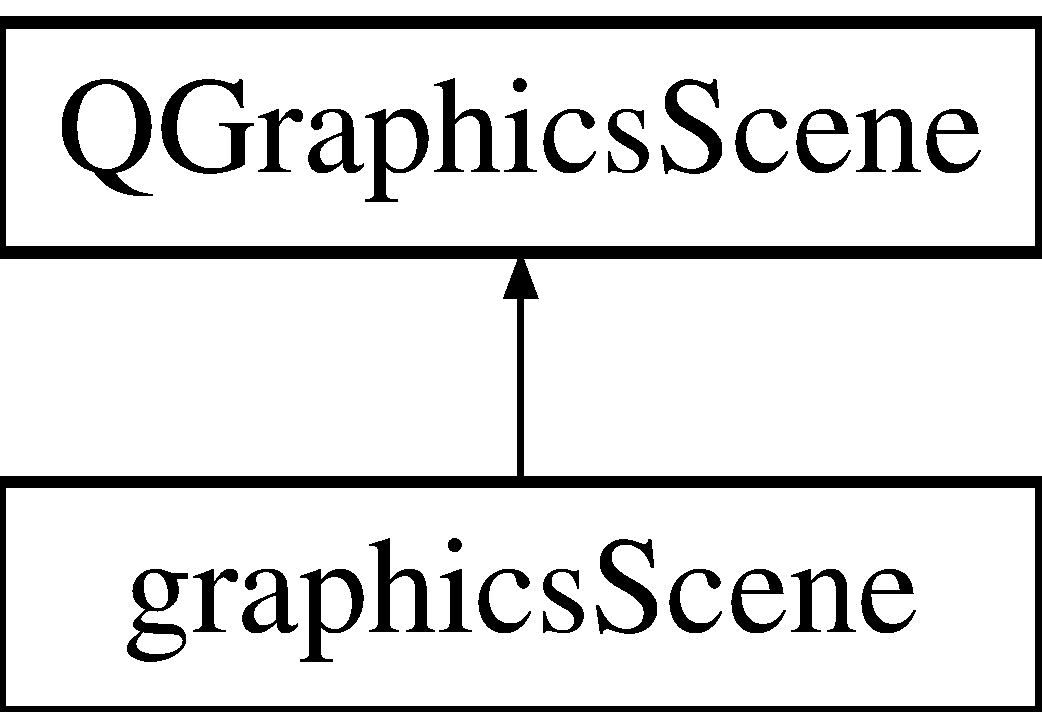
\includegraphics[height=2.000000cm]{classgraphics_scene}
\end{center}
\end{figure}
\subsection*{Signals}
\begin{DoxyCompactItemize}
\item 
\mbox{\Hypertarget{classgraphics_scene_a370117524f759425873aa2dd710958c0}\label{classgraphics_scene_a370117524f759425873aa2dd710958c0}} 
void {\bfseries new\+Mouse\+Left\+Press} (Q\+PointF \mbox{\hyperlink{classpoint}{point}})
\item 
\mbox{\Hypertarget{classgraphics_scene_a788bb2305e72c0deb7cd95a7e245b79a}\label{classgraphics_scene_a788bb2305e72c0deb7cd95a7e245b79a}} 
void {\bfseries new\+Mouse\+Right\+Press} (Q\+PointF \mbox{\hyperlink{classpoint}{point}})
\item 
\mbox{\Hypertarget{classgraphics_scene_ad79f731b826d93f3c84d55f8d411666c}\label{classgraphics_scene_ad79f731b826d93f3c84d55f8d411666c}} 
void {\bfseries new\+Mouse\+Hover} (Q\+PointF \mbox{\hyperlink{classpoint}{point}})
\item 
\mbox{\Hypertarget{classgraphics_scene_ab5dc117c8417d256b4cb9a01cbcd9509}\label{classgraphics_scene_ab5dc117c8417d256b4cb9a01cbcd9509}} 
void {\bfseries un\+Highlight\+Cycle} ()
\end{DoxyCompactItemize}
\subsection*{Public Member Functions}
\begin{DoxyCompactItemize}
\item 
\mbox{\hyperlink{classgraphics_scene_a630f565d827637e6f46f5ae2e786cd06}{graphics\+Scene}} (Q\+Object $\ast$parent=0)
\begin{DoxyCompactList}\small\item\em Scene Constructor. \end{DoxyCompactList}\item 
bool \mbox{\hyperlink{classgraphics_scene_ab84d166160c74279bae4f59c2ccac244}{get\+Point\+Is\+Highlighted}} ()
\begin{DoxyCompactList}\small\item\em \mbox{\hyperlink{classgraphics_scene_ab84d166160c74279bae4f59c2ccac244}{graphics\+Scene\+::get\+Point\+Is\+Highlighted}} getter for point\+Is\+Highlighted. \end{DoxyCompactList}\item 
void \mbox{\hyperlink{classgraphics_scene_a96915f909391e379b8c6c880d1d3acc6}{set\+Point\+Is\+Highlighted}} (const bool \&value)
\begin{DoxyCompactList}\small\item\em \mbox{\hyperlink{classgraphics_scene_a96915f909391e379b8c6c880d1d3acc6}{graphics\+Scene\+::set\+Point\+Is\+Highlighted}} setter for point\+Is\+Highlighted. \end{DoxyCompactList}\item 
virtual void \mbox{\hyperlink{classgraphics_scene_a45ca641319ec6accb1574f52539e7517}{mouse\+Press\+Event}} (Q\+Graphics\+Scene\+Mouse\+Event $\ast$mouse\+Event)
\begin{DoxyCompactList}\small\item\em \mbox{\hyperlink{classgraphics_scene_a45ca641319ec6accb1574f52539e7517}{graphics\+Scene\+::mouse\+Press\+Event}} Mouse pressed on scene \end{DoxyCompactList}\item 
virtual void \mbox{\hyperlink{classgraphics_scene_a08bfd268527873e3bccaa52f34823058}{mouse\+Move\+Event}} (Q\+Graphics\+Scene\+Mouse\+Event $\ast$mouse\+Event)
\begin{DoxyCompactList}\small\item\em \mbox{\hyperlink{classgraphics_scene_a08bfd268527873e3bccaa52f34823058}{graphics\+Scene\+::mouse\+Move\+Event}} Mouse moved on scene. \end{DoxyCompactList}\end{DoxyCompactItemize}


\subsection{Detailed Description}
The \mbox{\hyperlink{classgraphics_scene}{graphics\+Scene}} class. 

Scene displayed in the main part of the G\+UI. 

\subsection{Constructor \& Destructor Documentation}
\mbox{\Hypertarget{classgraphics_scene_a630f565d827637e6f46f5ae2e786cd06}\label{classgraphics_scene_a630f565d827637e6f46f5ae2e786cd06}} 
\index{graphics\+Scene@{graphics\+Scene}!graphics\+Scene@{graphics\+Scene}}
\index{graphics\+Scene@{graphics\+Scene}!graphics\+Scene@{graphics\+Scene}}
\subsubsection{\texorpdfstring{graphics\+Scene()}{graphicsScene()}}
{\footnotesize\ttfamily graphics\+Scene\+::graphics\+Scene (\begin{DoxyParamCaption}\item[{Q\+Object $\ast$}]{parent = {\ttfamily 0} }\end{DoxyParamCaption})\hspace{0.3cm}{\ttfamily [explicit]}}



Scene Constructor. 


\begin{DoxyParams}{Parameters}
{\em parent} & The parent widget to the current widget.\\
\hline
\end{DoxyParams}
Create a new scene setting the scene size to the predetermined size. 

\subsection{Member Function Documentation}
\mbox{\Hypertarget{classgraphics_scene_ab84d166160c74279bae4f59c2ccac244}\label{classgraphics_scene_ab84d166160c74279bae4f59c2ccac244}} 
\index{graphics\+Scene@{graphics\+Scene}!get\+Point\+Is\+Highlighted@{get\+Point\+Is\+Highlighted}}
\index{get\+Point\+Is\+Highlighted@{get\+Point\+Is\+Highlighted}!graphics\+Scene@{graphics\+Scene}}
\subsubsection{\texorpdfstring{get\+Point\+Is\+Highlighted()}{getPointIsHighlighted()}}
{\footnotesize\ttfamily bool graphics\+Scene\+::get\+Point\+Is\+Highlighted (\begin{DoxyParamCaption}{ }\end{DoxyParamCaption})}



\mbox{\hyperlink{classgraphics_scene_ab84d166160c74279bae4f59c2ccac244}{graphics\+Scene\+::get\+Point\+Is\+Highlighted}} getter for point\+Is\+Highlighted. 

\begin{DoxyReturn}{Returns}
bool
\end{DoxyReturn}
Point\+Is\+Highlighted represents a boolean value that determines if a point is being hovered or not. \mbox{\Hypertarget{classgraphics_scene_a08bfd268527873e3bccaa52f34823058}\label{classgraphics_scene_a08bfd268527873e3bccaa52f34823058}} 
\index{graphics\+Scene@{graphics\+Scene}!mouse\+Move\+Event@{mouse\+Move\+Event}}
\index{mouse\+Move\+Event@{mouse\+Move\+Event}!graphics\+Scene@{graphics\+Scene}}
\subsubsection{\texorpdfstring{mouse\+Move\+Event()}{mouseMoveEvent()}}
{\footnotesize\ttfamily void graphics\+Scene\+::mouse\+Move\+Event (\begin{DoxyParamCaption}\item[{Q\+Graphics\+Scene\+Mouse\+Event $\ast$}]{mouse\+Event }\end{DoxyParamCaption})\hspace{0.3cm}{\ttfamily [virtual]}}



\mbox{\hyperlink{classgraphics_scene_a08bfd268527873e3bccaa52f34823058}{graphics\+Scene\+::mouse\+Move\+Event}} Mouse moved on scene. 


\begin{DoxyParams}{Parameters}
{\em mouse\+Event} & Provides information about the mouse event such as the position the click occured on the scene.\\
\hline
\end{DoxyParams}
Called when the mouse moves over the scene. Signal is emitted to update coordinates on the status bar. \mbox{\Hypertarget{classgraphics_scene_a45ca641319ec6accb1574f52539e7517}\label{classgraphics_scene_a45ca641319ec6accb1574f52539e7517}} 
\index{graphics\+Scene@{graphics\+Scene}!mouse\+Press\+Event@{mouse\+Press\+Event}}
\index{mouse\+Press\+Event@{mouse\+Press\+Event}!graphics\+Scene@{graphics\+Scene}}
\subsubsection{\texorpdfstring{mouse\+Press\+Event()}{mousePressEvent()}}
{\footnotesize\ttfamily void graphics\+Scene\+::mouse\+Press\+Event (\begin{DoxyParamCaption}\item[{Q\+Graphics\+Scene\+Mouse\+Event $\ast$}]{mouse\+Event }\end{DoxyParamCaption})\hspace{0.3cm}{\ttfamily [virtual]}}



\mbox{\hyperlink{classgraphics_scene_a45ca641319ec6accb1574f52539e7517}{graphics\+Scene\+::mouse\+Press\+Event}} Mouse pressed on scene 


\begin{DoxyParams}{Parameters}
{\em mouse\+Event} & Provides information about the mouse event such as the position the click occured on the scene.\\
\hline
\end{DoxyParams}
Called when the mouse button is clicked on the scene in the graphics view. A left mouse click will mean a new point is created or the highlighted point is moved. A right mouse click will display the context menu. \mbox{\Hypertarget{classgraphics_scene_a96915f909391e379b8c6c880d1d3acc6}\label{classgraphics_scene_a96915f909391e379b8c6c880d1d3acc6}} 
\index{graphics\+Scene@{graphics\+Scene}!set\+Point\+Is\+Highlighted@{set\+Point\+Is\+Highlighted}}
\index{set\+Point\+Is\+Highlighted@{set\+Point\+Is\+Highlighted}!graphics\+Scene@{graphics\+Scene}}
\subsubsection{\texorpdfstring{set\+Point\+Is\+Highlighted()}{setPointIsHighlighted()}}
{\footnotesize\ttfamily void graphics\+Scene\+::set\+Point\+Is\+Highlighted (\begin{DoxyParamCaption}\item[{const bool \&}]{value }\end{DoxyParamCaption})}



\mbox{\hyperlink{classgraphics_scene_a96915f909391e379b8c6c880d1d3acc6}{graphics\+Scene\+::set\+Point\+Is\+Highlighted}} setter for point\+Is\+Highlighted. 


\begin{DoxyParams}{Parameters}
{\em value} & Point\+Is\+Highlighted represents a boolean value that determines if a point is being hovered or not. \\
\hline
\end{DoxyParams}


The documentation for this class was generated from the following files\+:\begin{DoxyCompactItemize}
\item 
/\+Users/lukehutton/\+One\+Drive -\/ University of Leeds/\+University/\+Computer Science/\+Internship/moebinv-\/gui/include/scene.\+h\item 
/\+Users/lukehutton/\+One\+Drive -\/ University of Leeds/\+University/\+Computer Science/\+Internship/moebinv-\/gui/moebinv-\/gui-\/build/moc\+\_\+scene.\+cpp\item 
/\+Users/lukehutton/\+One\+Drive -\/ University of Leeds/\+University/\+Computer Science/\+Internship/moebinv-\/gui/src/scene.\+cpp\end{DoxyCompactItemize}

\hypertarget{classlabels}{}\section{labels Class Reference}
\label{classlabels}\index{labels@{labels}}


The labels class.  




{\ttfamily \#include $<$labels.\+h$>$}

\subsection*{Public Member Functions}
\begin{DoxyCompactItemize}
\item 
\mbox{\Hypertarget{classlabels_aabee553ffee5eb33826c90bbda2dbc58}\label{classlabels_aabee553ffee5eb33826c90bbda2dbc58}} 
\mbox{\hyperlink{classlabels_aabee553ffee5eb33826c90bbda2dbc58}{labels}} ()
\begin{DoxyCompactList}\small\item\em \mbox{\hyperlink{classlabels_aabee553ffee5eb33826c90bbda2dbc58}{labels\+::labels}} Labels constructor. \end{DoxyCompactList}\item 
Q\+String \mbox{\hyperlink{classlabels_a70a7436dbef91e342fec4ec3130187e2}{gen\+Next\+Label}} ()
\begin{DoxyCompactList}\small\item\em \mbox{\hyperlink{classlabels_a70a7436dbef91e342fec4ec3130187e2}{labels\+::gen\+Next\+Label}} Generate next label. \end{DoxyCompactList}\item 
\mbox{\Hypertarget{classlabels_a790344f0c86546b9b5fdda30dbe690a5}\label{classlabels_a790344f0c86546b9b5fdda30dbe690a5}} 
void {\bfseries advance\+Label} ()
\end{DoxyCompactItemize}


\subsection{Detailed Description}
The labels class. 

The labels class is a small class which generates a unique label incrementing as such\+: A, B, C, ..., Z, AA, AB, ... ZZ, A\+AA, ect... 

\subsection{Member Function Documentation}
\mbox{\Hypertarget{classlabels_a70a7436dbef91e342fec4ec3130187e2}\label{classlabels_a70a7436dbef91e342fec4ec3130187e2}} 
\index{labels@{labels}!gen\+Next\+Label@{gen\+Next\+Label}}
\index{gen\+Next\+Label@{gen\+Next\+Label}!labels@{labels}}
\subsubsection{\texorpdfstring{gen\+Next\+Label()}{genNextLabel()}}
{\footnotesize\ttfamily Q\+String labels\+::gen\+Next\+Label (\begin{DoxyParamCaption}{ }\end{DoxyParamCaption})}



\mbox{\hyperlink{classlabels_a70a7436dbef91e342fec4ec3130187e2}{labels\+::gen\+Next\+Label}} Generate next label. 

\begin{DoxyReturn}{Returns}
New label.
\end{DoxyReturn}
Generate the next label in the sequence i.\+e. A, B, C, ..., Z, AA, AB, ... 

The documentation for this class was generated from the following files\+:\begin{DoxyCompactItemize}
\item 
/\+Users/lukehutton/\+One\+Drive -\/ University of Leeds/\+University/\+Computer Science/\+Internship/moebinv-\/gui/include/labels.\+h\item 
/\+Users/lukehutton/\+One\+Drive -\/ University of Leeds/\+University/\+Computer Science/\+Internship/moebinv-\/gui/src/labels.\+cpp\end{DoxyCompactItemize}

\hypertarget{classline}{}\section{line Class Reference}
\label{classline}\index{line@{line}}
Inheritance diagram for line\+:\begin{figure}[H]
\begin{center}
\leavevmode
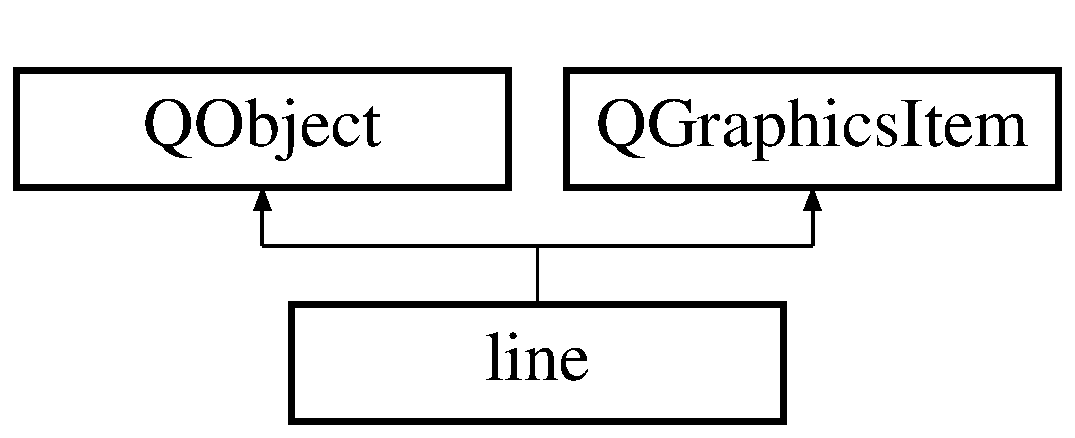
\includegraphics[height=2.000000cm]{classline}
\end{center}
\end{figure}
\subsection*{Public Member Functions}
\begin{DoxyCompactItemize}
\item 
\mbox{\hyperlink{classline_a38ef6d493f122a35237517bc79653821}{line}} (\mbox{\hyperlink{classgraphic_cycle}{graphic\+Cycle}} $\ast$parent, struct \mbox{\hyperlink{structcycle_data}{cycle\+Data}} data)
\begin{DoxyCompactList}\small\item\em \mbox{\hyperlink{classline_a38ef6d493f122a35237517bc79653821}{line\+::line}} Create a new line. \end{DoxyCompactList}\item 
void \mbox{\hyperlink{classline_a128cee38b49baa22b618165edc900e81}{paint}} (Q\+Painter $\ast$painter, const Q\+Style\+Option\+Graphics\+Item $\ast$option, Q\+Widget $\ast$widget)
\begin{DoxyCompactList}\small\item\em \mbox{\hyperlink{classline_a128cee38b49baa22b618165edc900e81}{line\+::paint}} Paint the point on the scene. \end{DoxyCompactList}\item 
Q\+RectF \mbox{\hyperlink{classline_aecbda133a991abe5bb4080416c226e2f}{bounding\+Rect}} () const
\begin{DoxyCompactList}\small\item\em \mbox{\hyperlink{classline_aecbda133a991abe5bb4080416c226e2f}{line\+::bounding\+Rect}} Define the bounding rect. \end{DoxyCompactList}\item 
void \mbox{\hyperlink{classline_a0638608cbb7231dc4a55ea795e367748}{find\+Line\+Points}} ()
\begin{DoxyCompactList}\small\item\em line\+::shape Define the clipping mask of the object \end{DoxyCompactList}\end{DoxyCompactItemize}


\subsection{Constructor \& Destructor Documentation}
\mbox{\Hypertarget{classline_a38ef6d493f122a35237517bc79653821}\label{classline_a38ef6d493f122a35237517bc79653821}} 
\index{line@{line}!line@{line}}
\index{line@{line}!line@{line}}
\subsubsection{\texorpdfstring{line()}{line()}}
{\footnotesize\ttfamily line\+::line (\begin{DoxyParamCaption}\item[{\mbox{\hyperlink{classgraphic_cycle}{graphic\+Cycle}} $\ast$}]{parent,  }\item[{struct \mbox{\hyperlink{structcycle_data}{cycle\+Data}}}]{data }\end{DoxyParamCaption})}



\mbox{\hyperlink{classline_a38ef6d493f122a35237517bc79653821}{line\+::line}} Create a new line. 


\begin{DoxyParams}{Parameters}
{\em struct} & \mbox{\hyperlink{structcycle_data}{cycle\+Data}} data Contains the data needed to draw the line.\\
\hline
\end{DoxyParams}
Construct a new line on the scene and assign it to the parent \mbox{\hyperlink{classgraphic_cycle}{graphic\+Cycle}}. 

\subsection{Member Function Documentation}
\mbox{\Hypertarget{classline_aecbda133a991abe5bb4080416c226e2f}\label{classline_aecbda133a991abe5bb4080416c226e2f}} 
\index{line@{line}!bounding\+Rect@{bounding\+Rect}}
\index{bounding\+Rect@{bounding\+Rect}!line@{line}}
\subsubsection{\texorpdfstring{bounding\+Rect()}{boundingRect()}}
{\footnotesize\ttfamily Q\+RectF line\+::bounding\+Rect (\begin{DoxyParamCaption}{ }\end{DoxyParamCaption}) const}



\mbox{\hyperlink{classline_aecbda133a991abe5bb4080416c226e2f}{line\+::bounding\+Rect}} Define the bounding rect. 

\begin{DoxyReturn}{Returns}
Q\+RectF
\end{DoxyReturn}
Define the box the object is drawn within on the scene. \mbox{\Hypertarget{classline_a0638608cbb7231dc4a55ea795e367748}\label{classline_a0638608cbb7231dc4a55ea795e367748}} 
\index{line@{line}!find\+Line\+Points@{find\+Line\+Points}}
\index{find\+Line\+Points@{find\+Line\+Points}!line@{line}}
\subsubsection{\texorpdfstring{find\+Line\+Points()}{findLinePoints()}}
{\footnotesize\ttfamily void line\+::find\+Line\+Points (\begin{DoxyParamCaption}{ }\end{DoxyParamCaption})}



line\+::shape Define the clipping mask of the object 

\begin{DoxyReturn}{Returns}
Q\+Painter\+Path
\end{DoxyReturn}
Defines the area in which the shape actually exists.

\mbox{\hyperlink{classline_a0638608cbb7231dc4a55ea795e367748}{line\+::find\+Line\+Points}} Find the points\+: (x1, y1), (x2, y2).

This function finds the two points in which the line will be drawn between. Hence since we need to draw a line accross the whole of the scene, we find two points which are beyond the scene and draw the line between those. \mbox{\Hypertarget{classline_a128cee38b49baa22b618165edc900e81}\label{classline_a128cee38b49baa22b618165edc900e81}} 
\index{line@{line}!paint@{paint}}
\index{paint@{paint}!line@{line}}
\subsubsection{\texorpdfstring{paint()}{paint()}}
{\footnotesize\ttfamily void line\+::paint (\begin{DoxyParamCaption}\item[{Q\+Painter $\ast$}]{painter,  }\item[{const Q\+Style\+Option\+Graphics\+Item $\ast$}]{option,  }\item[{Q\+Widget $\ast$}]{widget }\end{DoxyParamCaption})}



\mbox{\hyperlink{classline_a128cee38b49baa22b618165edc900e81}{line\+::paint}} Paint the point on the scene. 


\begin{DoxyParams}{Parameters}
{\em p} & Q\+Painter object. \\
\hline
{\em option} & \\
\hline
{\em widget} & This function paints the line on the scene given various parameters (such as x and y). The line is drawn differently dependent on the drawing metric in use. \\
\hline
\end{DoxyParams}


The documentation for this class was generated from the following files\+:\begin{DoxyCompactItemize}
\item 
/\+Users/lukehutton/\+One\+Drive -\/ University of Leeds/\+University/\+Computer Science/\+Internship/moebinv-\/gui/include/line.\+h\item 
/\+Users/lukehutton/\+One\+Drive -\/ University of Leeds/\+University/\+Computer Science/\+Internship/moebinv-\/gui/src/line.\+cpp\end{DoxyCompactItemize}

\hypertarget{class_main_window}{}\section{Main\+Window Class Reference}
\label{class_main_window}\index{Main\+Window@{Main\+Window}}


The \mbox{\hyperlink{class_main_window}{Main\+Window}} class.  




{\ttfamily \#include $<$mainwindow.\+h$>$}

Inheritance diagram for Main\+Window\+:\begin{figure}[H]
\begin{center}
\leavevmode
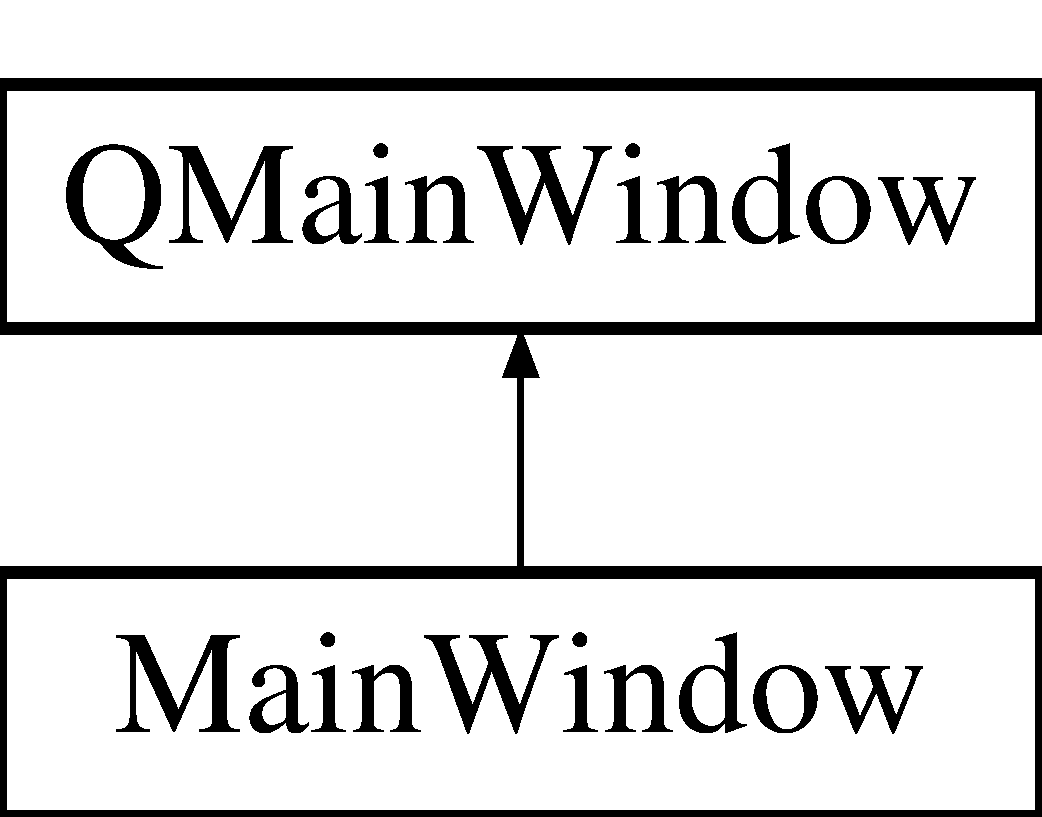
\includegraphics[height=2.000000cm]{class_main_window}
\end{center}
\end{figure}
\subsection*{Signals}
\begin{DoxyCompactItemize}
\item 
\mbox{\Hypertarget{class_main_window_a46ebd786b1aeb0ef026f0a3f32dd9f3d}\label{class_main_window_a46ebd786b1aeb0ef026f0a3f32dd9f3d}} 
void {\bfseries reset\+Relational\+List} ()
\end{DoxyCompactItemize}
\subsection*{Public Member Functions}
\begin{DoxyCompactItemize}
\item 
\mbox{\hyperlink{class_main_window_a8b244be8b7b7db1b08de2a2acb9409db}{Main\+Window}} (Q\+Widget $\ast$parent=0)
\begin{DoxyCompactList}\small\item\em \mbox{\hyperlink{class_main_window_a8b244be8b7b7db1b08de2a2acb9409db}{Main\+Window\+::\+Main\+Window}}. \end{DoxyCompactList}\item 
void \mbox{\hyperlink{class_main_window_ad0adb1cd734f6bba159f13fd332d62f5}{init\+Figure}} ()
\begin{DoxyCompactList}\small\item\em \mbox{\hyperlink{class_main_window_ad0adb1cd734f6bba159f13fd332d62f5}{Main\+Window\+::init\+Figure}} Initialize figure. \end{DoxyCompactList}\item 
void \mbox{\hyperlink{class_main_window_aa33398d6788bcd727486b5fff5c238e4}{add\+Point}} (Q\+PointF location)
\begin{DoxyCompactList}\small\item\em Main\+Window\+::add\+Cycle Add a cycle to the figure. \end{DoxyCompactList}\item 
\mbox{\Hypertarget{class_main_window_af7d2eb4ee3fb3cc4f0b83deffdb81ae8}\label{class_main_window_af7d2eb4ee3fb3cc4f0b83deffdb81ae8}} 
void {\bfseries set\+Drawing\+Metric} ()
\item 
\mbox{\Hypertarget{class_main_window_a40346d328146b3a78cb08a400c53a47e}\label{class_main_window_a40346d328146b3a78cb08a400c53a47e}} 
void {\bfseries add\+Point\+To\+Tree} (\mbox{\hyperlink{classpoint}{point}} $\ast$p)
\item 
\mbox{\Hypertarget{class_main_window_ad322f29d75b06348ee43ce911a1cc36f}\label{class_main_window_ad322f29d75b06348ee43ce911a1cc36f}} 
void {\bfseries add\+Line\+To\+Tree} (Q\+String item\+Name)
\item 
\mbox{\Hypertarget{class_main_window_aac80f9ac141e25d2fae5ae71ba762142}\label{class_main_window_aac80f9ac141e25d2fae5ae71ba762142}} 
void {\bfseries add\+Cycle\+To\+Tree} (\mbox{\hyperlink{classcircle}{circle}} $\ast$c)
\item 
\mbox{\Hypertarget{class_main_window_ac993682874f221dbe0e82c7118d05684}\label{class_main_window_ac993682874f221dbe0e82c7118d05684}} 
void {\bfseries reset\+List} (Gi\+Na\+C\+::lst $\ast$list)
\item 
\mbox{\Hypertarget{class_main_window_a3e45090789e16c49079857ab0617b239}\label{class_main_window_a3e45090789e16c49079857ab0617b239}} 
void {\bfseries init\+Tree\+Model} ()
\item 
\mbox{\Hypertarget{class_main_window_ae78352e402084a7c6518e97056070677}\label{class_main_window_ae78352e402084a7c6518e97056070677}} 
void {\bfseries init\+Main\+Menu} ()
\item 
\mbox{\Hypertarget{class_main_window_ae98d00a93bc118200eeef9f9bba1dba7}\label{class_main_window_ae98d00a93bc118200eeef9f9bba1dba7}} 
\mbox{\hyperlink{class_main_window_ae98d00a93bc118200eeef9f9bba1dba7}{$\sim$\+Main\+Window}} ()
\begin{DoxyCompactList}\small\item\em \mbox{\hyperlink{class_main_window_ae98d00a93bc118200eeef9f9bba1dba7}{Main\+Window\+::$\sim$\+Main\+Window}} \mbox{\hyperlink{class_main_window}{Main\+Window}} destructor. \end{DoxyCompactList}\end{DoxyCompactItemize}
\subsection*{Public Attributes}
\begin{DoxyCompactItemize}
\item 
\mbox{\Hypertarget{class_main_window_ada1631bee647fb176facf5077da7f91c}\label{class_main_window_ada1631bee647fb176facf5077da7f91c}} 
bool {\bfseries tool\+Add\+Cycle}
\end{DoxyCompactItemize}


\subsection{Detailed Description}
The \mbox{\hyperlink{class_main_window}{Main\+Window}} class. 

\mbox{\hyperlink{class_main_window}{Main\+Window}}, the main application. This encompasses the scene, menu and tree view. 

\subsection{Constructor \& Destructor Documentation}
\mbox{\Hypertarget{class_main_window_a8b244be8b7b7db1b08de2a2acb9409db}\label{class_main_window_a8b244be8b7b7db1b08de2a2acb9409db}} 
\index{Main\+Window@{Main\+Window}!Main\+Window@{Main\+Window}}
\index{Main\+Window@{Main\+Window}!Main\+Window@{Main\+Window}}
\subsubsection{\texorpdfstring{Main\+Window()}{MainWindow()}}
{\footnotesize\ttfamily Main\+Window\+::\+Main\+Window (\begin{DoxyParamCaption}\item[{Q\+Widget $\ast$}]{parent = {\ttfamily 0} }\end{DoxyParamCaption})\hspace{0.3cm}{\ttfamily [explicit]}}



\mbox{\hyperlink{class_main_window_a8b244be8b7b7db1b08de2a2acb9409db}{Main\+Window\+::\+Main\+Window}}. 


\begin{DoxyParams}{Parameters}
{\em parent} & \\
\hline
\end{DoxyParams}


\subsection{Member Function Documentation}
\mbox{\Hypertarget{class_main_window_aa33398d6788bcd727486b5fff5c238e4}\label{class_main_window_aa33398d6788bcd727486b5fff5c238e4}} 
\index{Main\+Window@{Main\+Window}!add\+Point@{add\+Point}}
\index{add\+Point@{add\+Point}!Main\+Window@{Main\+Window}}
\subsubsection{\texorpdfstring{add\+Point()}{addPoint()}}
{\footnotesize\ttfamily void Main\+Window\+::add\+Point (\begin{DoxyParamCaption}\item[{Q\+PointF}]{mouse\+Pos }\end{DoxyParamCaption})}



Main\+Window\+::add\+Cycle Add a cycle to the figure. 


\begin{DoxyParams}{Parameters}
{\em mouse\+Pos} & Coordinates of mouse on the scene.\\
\hline
\end{DoxyParams}
Adds a cycle to the figure then draws it on the scene. \mbox{\Hypertarget{class_main_window_ad0adb1cd734f6bba159f13fd332d62f5}\label{class_main_window_ad0adb1cd734f6bba159f13fd332d62f5}} 
\index{Main\+Window@{Main\+Window}!init\+Figure@{init\+Figure}}
\index{init\+Figure@{init\+Figure}!Main\+Window@{Main\+Window}}
\subsubsection{\texorpdfstring{init\+Figure()}{initFigure()}}
{\footnotesize\ttfamily void Main\+Window\+::init\+Figure (\begin{DoxyParamCaption}{ }\end{DoxyParamCaption})}



\mbox{\hyperlink{class_main_window_ad0adb1cd734f6bba159f13fd332d62f5}{Main\+Window\+::init\+Figure}} Initialize figure. 

Create a new figure and apply any additional settings. 

The documentation for this class was generated from the following files\+:\begin{DoxyCompactItemize}
\item 
/\+Users/lukehutton/\+One\+Drive -\/ University of Leeds/\+University/\+Computer Science/\+Internship/moebinv-\/gui/include/mainwindow.\+h\item 
/\+Users/lukehutton/\+One\+Drive -\/ University of Leeds/\+University/\+Computer Science/\+Internship/moebinv-\/gui/src/mainwindow.\+cpp\end{DoxyCompactItemize}

\hypertarget{classpoint}{}\section{point Class Reference}
\label{classpoint}\index{point@{point}}


The point class.  




{\ttfamily \#include $<$point.\+h$>$}

Inheritance diagram for point\+:\begin{figure}[H]
\begin{center}
\leavevmode
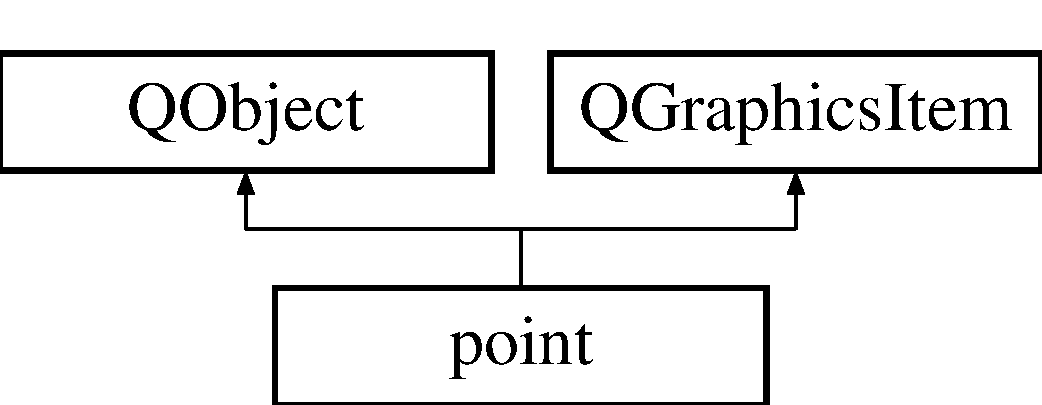
\includegraphics[height=3.000000cm]{classpoint}
\end{center}
\end{figure}
\subsection*{Public Member Functions}
\begin{DoxyCompactItemize}
\item 
\mbox{\hyperlink{classpoint_aabf8c59fffa6fb48ac1d9bcec101c3aa}{point}} (Moeb\+Inv\+::figure $\ast$f, Gi\+Na\+C\+::ex p, Q\+String l, int z)
\begin{DoxyCompactList}\small\item\em \mbox{\hyperlink{classpoint_aabf8c59fffa6fb48ac1d9bcec101c3aa}{point\+::point}} Point constructor. \end{DoxyCompactList}\item 
void \mbox{\hyperlink{classpoint_a5e75bab386500018e5d068c920ed0e66}{paint}} (Q\+Painter $\ast$p, const Q\+Style\+Option\+Graphics\+Item $\ast$, Q\+Widget $\ast$)
\begin{DoxyCompactList}\small\item\em \mbox{\hyperlink{classpoint_a5e75bab386500018e5d068c920ed0e66}{point\+::paint}} Paint the point on the scene. \end{DoxyCompactList}\item 
Q\+RectF \mbox{\hyperlink{classpoint_a91a81fc826052833e19e9d39ef3849d9}{bounding\+Rect}} () const
\begin{DoxyCompactList}\small\item\em \mbox{\hyperlink{classpoint_a91a81fc826052833e19e9d39ef3849d9}{point\+::bounding\+Rect}} Define the bounding rectangle \end{DoxyCompactList}\end{DoxyCompactItemize}
\subsection*{Additional Inherited Members}


\subsection{Detailed Description}
The point class. 

When created and added to the scene a point is displayed, given the x coordinate and y coordinates.

Inherits \mbox{\hyperlink{classgraphic_cycle}{graphic\+Cycle}}. 

\subsection{Constructor \& Destructor Documentation}
\mbox{\Hypertarget{classpoint_aabf8c59fffa6fb48ac1d9bcec101c3aa}\label{classpoint_aabf8c59fffa6fb48ac1d9bcec101c3aa}} 
\index{point@{point}!point@{point}}
\index{point@{point}!point@{point}}
\subsubsection{\texorpdfstring{point()}{point()}}
{\footnotesize\ttfamily point\+::point (\begin{DoxyParamCaption}\item[{Moeb\+Inv\+::figure $\ast$}]{f,  }\item[{Gi\+Na\+C\+::ex}]{p,  }\item[{Q\+String}]{l,  }\item[{int}]{z }\end{DoxyParamCaption})\hspace{0.3cm}{\ttfamily [explicit]}}



\mbox{\hyperlink{classpoint_aabf8c59fffa6fb48ac1d9bcec101c3aa}{point\+::point}} Point constructor. 


\begin{DoxyParams}{Parameters}
{\em f} & Moeb\+Inv figure. \\
\hline
{\em p} & Moeb\+Inv point to be drawn on the scene. \\
\hline
{\em l} & label of the point. \\
\hline
{\em z} & index in which to draw the object. \\
\hline
{\em parent} & Constructs a point on the scene.\\
\hline
\end{DoxyParams}
Inherits \textquotesingle{}\mbox{\hyperlink{classgraphic_cycle}{graphic\+Cycle}}\textquotesingle{}. 

\subsection{Member Function Documentation}
\mbox{\Hypertarget{classpoint_a91a81fc826052833e19e9d39ef3849d9}\label{classpoint_a91a81fc826052833e19e9d39ef3849d9}} 
\index{point@{point}!bounding\+Rect@{bounding\+Rect}}
\index{bounding\+Rect@{bounding\+Rect}!point@{point}}
\subsubsection{\texorpdfstring{bounding\+Rect()}{boundingRect()}}
{\footnotesize\ttfamily Q\+RectF point\+::bounding\+Rect (\begin{DoxyParamCaption}{ }\end{DoxyParamCaption}) const\hspace{0.3cm}{\ttfamily [virtual]}}



\mbox{\hyperlink{classpoint_a91a81fc826052833e19e9d39ef3849d9}{point\+::bounding\+Rect}} Define the bounding rectangle 

\begin{DoxyReturn}{Returns}
Q\+RectF
\end{DoxyReturn}
Defines the area on the scene that the object can draw on. 

Implements \mbox{\hyperlink{classgraphic_cycle}{graphic\+Cycle}}.

\mbox{\Hypertarget{classpoint_a5e75bab386500018e5d068c920ed0e66}\label{classpoint_a5e75bab386500018e5d068c920ed0e66}} 
\index{point@{point}!paint@{paint}}
\index{paint@{paint}!point@{point}}
\subsubsection{\texorpdfstring{paint()}{paint()}}
{\footnotesize\ttfamily void point\+::paint (\begin{DoxyParamCaption}\item[{Q\+Painter $\ast$}]{p,  }\item[{const Q\+Style\+Option\+Graphics\+Item $\ast$}]{,  }\item[{Q\+Widget $\ast$}]{ }\end{DoxyParamCaption})\hspace{0.3cm}{\ttfamily [virtual]}}



\mbox{\hyperlink{classpoint_a5e75bab386500018e5d068c920ed0e66}{point\+::paint}} Paint the point on the scene. 


\begin{DoxyParams}{Parameters}
{\em p} & Q\+Painter object.\\
\hline
\end{DoxyParams}
This function paints the point on the scene given various parameters (such as x, y, radius and label). The point is drawn differently dependent on the drawing metric in use. 

Implements \mbox{\hyperlink{classgraphic_cycle}{graphic\+Cycle}}.



The documentation for this class was generated from the following files\+:\begin{DoxyCompactItemize}
\item 
/\+Users/lukehutton/\+One\+Drive -\/ University of Leeds/\+University/\+Computer Science/\+Internship/moebinv-\/gui/include/point.\+h\item 
/\+Users/lukehutton/\+One\+Drive -\/ University of Leeds/\+University/\+Computer Science/\+Internship/moebinv-\/gui/src/point.\+cpp\end{DoxyCompactItemize}

\hypertarget{classtree_model}{}\section{tree\+Model Class Reference}
\label{classtree_model}\index{tree\+Model@{tree\+Model}}
Inheritance diagram for tree\+Model\+:\begin{figure}[H]
\begin{center}
\leavevmode
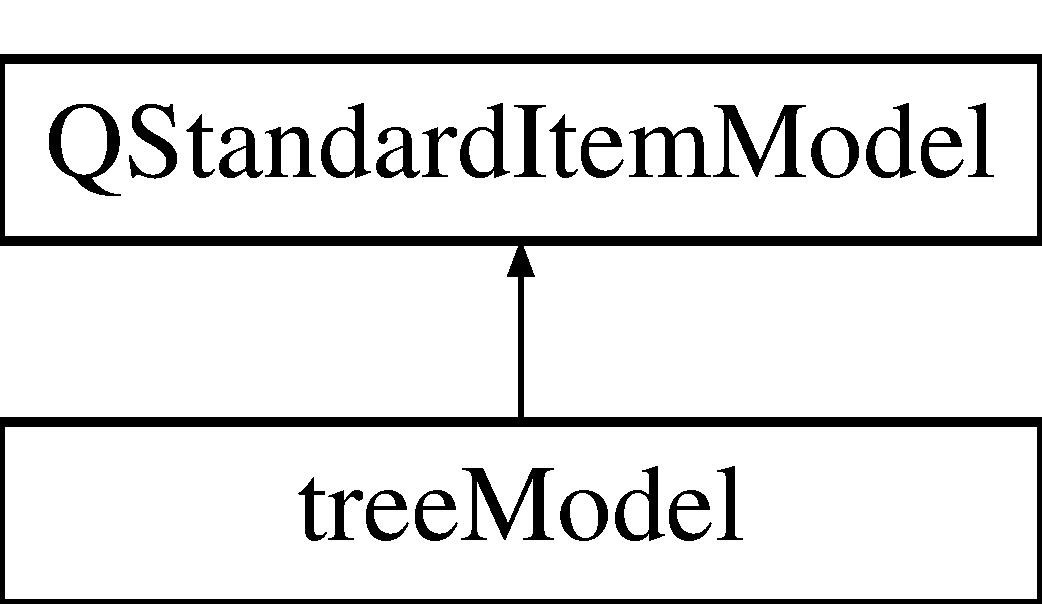
\includegraphics[height=2.000000cm]{classtree_model}
\end{center}
\end{figure}
\subsection*{Public Member Functions}
\begin{DoxyCompactItemize}
\item 
\mbox{\Hypertarget{classtree_model_ad3539d2628250edeea80fe4ffe0a80fa}\label{classtree_model_ad3539d2628250edeea80fe4ffe0a80fa}} 
{\bfseries tree\+Model} (Q\+Object $\ast$parent=0)
\end{DoxyCompactItemize}


The documentation for this class was generated from the following files\+:\begin{DoxyCompactItemize}
\item 
/\+Users/lukehutton/\+One\+Drive -\/ University of Leeds/\+University/\+Computer Science/\+Internship/moebinv-\/gui/include/treemodel.\+h\item 
/\+Users/lukehutton/\+One\+Drive -\/ University of Leeds/\+University/\+Computer Science/\+Internship/moebinv-\/gui/src/treemodel.\+cpp\end{DoxyCompactItemize}

\hypertarget{classzoom}{}\section{zoom Class Reference}
\label{classzoom}\index{zoom@{zoom}}


{\ttfamily \#include $<$zoom.\+h$>$}

Inheritance diagram for zoom\+:\begin{figure}[H]
\begin{center}
\leavevmode
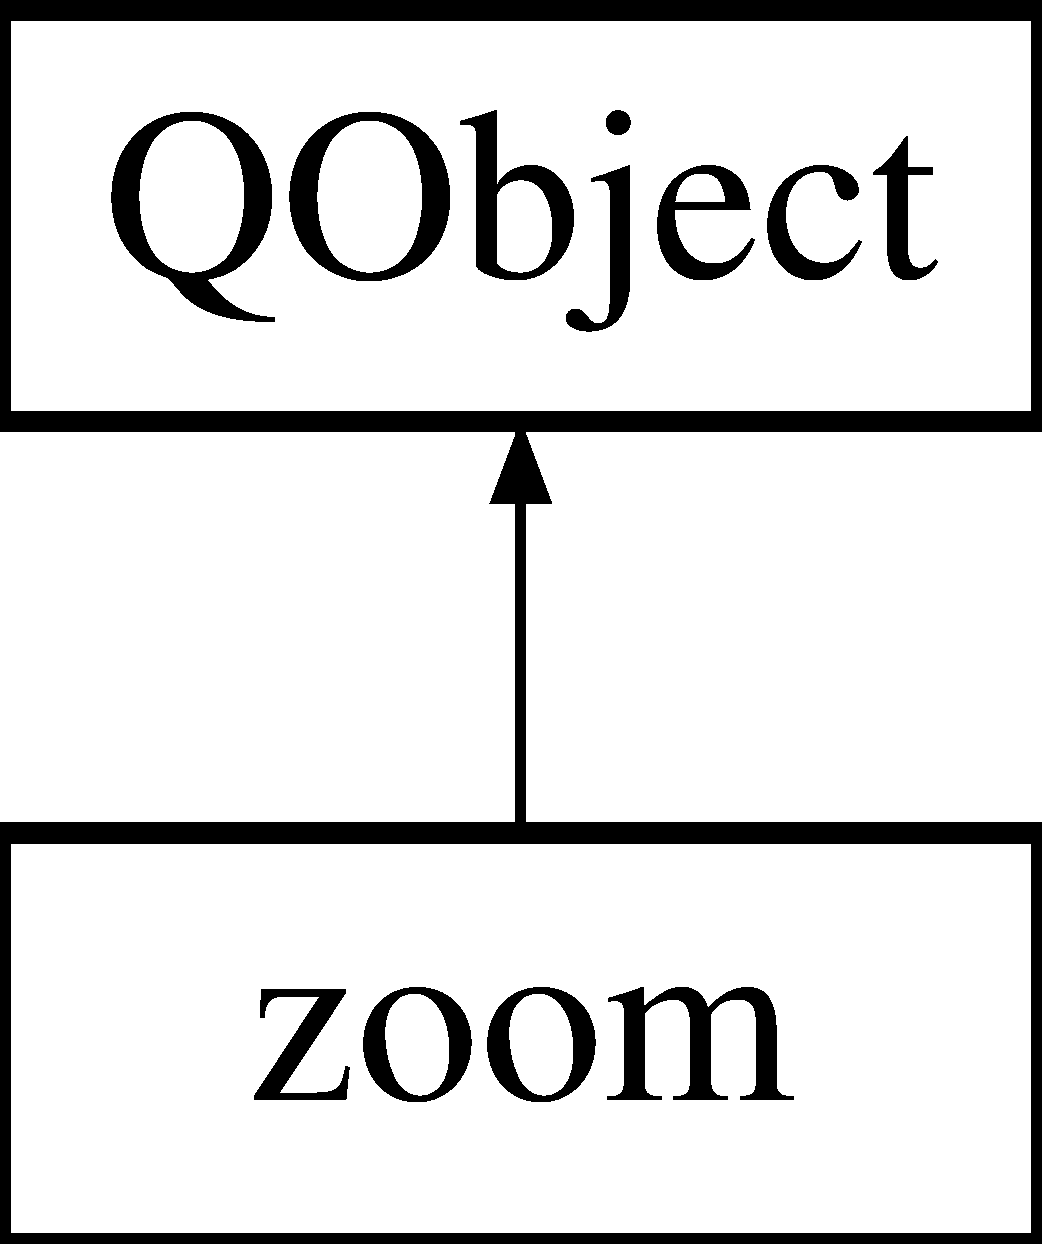
\includegraphics[height=2.000000cm]{classzoom}
\end{center}
\end{figure}
\subsection*{Signals}
\begin{DoxyCompactItemize}
\item 
\mbox{\Hypertarget{classzoom_adb6956b53b9e64ca1ccb0f46cbe3a35f}\label{classzoom_adb6956b53b9e64ca1ccb0f46cbe3a35f}} 
void {\bfseries zoomed} ()
\end{DoxyCompactItemize}
\subsection*{Public Member Functions}
\begin{DoxyCompactItemize}
\item 
\mbox{\Hypertarget{classzoom_a07440bd0b04ea8cb0ebf4b7add046ebe}\label{classzoom_a07440bd0b04ea8cb0ebf4b7add046ebe}} 
{\bfseries zoom} (Q\+Graphics\+View $\ast$view)
\item 
\mbox{\Hypertarget{classzoom_ac4d5419f79b8ffb9a51eaed182e9dd95}\label{classzoom_ac4d5419f79b8ffb9a51eaed182e9dd95}} 
void {\bfseries gentle\+\_\+zoom} (double factor)
\item 
\mbox{\Hypertarget{classzoom_a9efd3e68e59ebbffddffbeeec316be82}\label{classzoom_a9efd3e68e59ebbffddffbeeec316be82}} 
void {\bfseries set\+\_\+modifiers} (Qt\+::\+Keyboard\+Modifiers modifiers)
\item 
\mbox{\Hypertarget{classzoom_a2de8b7b8b6803586d41ce1f7b3864b77}\label{classzoom_a2de8b7b8b6803586d41ce1f7b3864b77}} 
void {\bfseries set\+\_\+zoom\+\_\+factor\+\_\+base} (double value)
\end{DoxyCompactItemize}


\subsection{Detailed Description}
This class adds ability to zoom Q\+Graphics\+View using mouse wheel. The point under cursor remains motionless while it\textquotesingle{}s possible.

Note that it becomes not possible when the scene\textquotesingle{}s size is not large enough comparing to the viewport size. Q\+Graphics\+View centers the picture when it\textquotesingle{}s smaller than the view. And Q\+Graphics\+View\textquotesingle{}s scrolls boundaries don\textquotesingle{}t allow to put any picture point at any viewport position.

When the user starts scrolling, this class remembers original scene position and keeps it until scrolling is completed. It\textquotesingle{}s better than getting original scene position at each scrolling step because that approach leads to position errors due to before-\/mentioned positioning restrictions.

When zommed using scroll, this class emits zoomed() signal.

Usage\+:

new Graphics\+\_\+view\+\_\+zoom(view);

The object will be deleted automatically when the view is deleted.

You can set keyboard modifiers used for zooming using set\+\_\+modified(). Zooming will be performed only on exact match of modifiers combination. The default modifier is Ctrl.

You can change zoom velocity by calling set\+\_\+zoom\+\_\+factor\+\_\+base(). Zoom coefficient is calculated as zoom\+\_\+factor\+\_\+base$^\wedge$angle\+\_\+delta (see Q\+Wheel\+Event\+::angle\+Delta). The default zoom factor base is 1.\+0015. 

The documentation for this class was generated from the following files\+:\begin{DoxyCompactItemize}
\item 
/\+Users/lukehutton/\+One\+Drive -\/ University of Leeds/\+University/\+Computer Science/\+Internship/moebinv-\/gui/include/zoom.\+h\item 
/\+Users/lukehutton/\+One\+Drive -\/ University of Leeds/\+University/\+Computer Science/\+Internship/moebinv-\/gui/src/zoom.\+cpp\end{DoxyCompactItemize}

%--- End generated contents ---

% Index
\backmatter
\newpage
\phantomsection
\clearemptydoublepage
\addcontentsline{toc}{chapter}{\indexname}
\printindex

\end{document}
